% Options for packages loaded elsewhere
\PassOptionsToPackage{unicode}{hyperref}
\PassOptionsToPackage{hyphens}{url}
%
\documentclass[
]{article}
\usepackage{amsmath,amssymb}
\usepackage{lmodern}
\usepackage{iftex}
\ifPDFTeX
  \usepackage[T1]{fontenc}
  \usepackage[utf8]{inputenc}
  \usepackage{textcomp} % provide euro and other symbols
\else % if luatex or xetex
  \usepackage{unicode-math}
  \defaultfontfeatures{Scale=MatchLowercase}
  \defaultfontfeatures[\rmfamily]{Ligatures=TeX,Scale=1}
\fi
% Use upquote if available, for straight quotes in verbatim environments
\IfFileExists{upquote.sty}{\usepackage{upquote}}{}
\IfFileExists{microtype.sty}{% use microtype if available
  \usepackage[]{microtype}
  \UseMicrotypeSet[protrusion]{basicmath} % disable protrusion for tt fonts
}{}
\makeatletter
\@ifundefined{KOMAClassName}{% if non-KOMA class
  \IfFileExists{parskip.sty}{%
    \usepackage{parskip}
  }{% else
    \setlength{\parindent}{0pt}
    \setlength{\parskip}{6pt plus 2pt minus 1pt}}
}{% if KOMA class
  \KOMAoptions{parskip=half}}
\makeatother
\usepackage{xcolor}
\IfFileExists{xurl.sty}{\usepackage{xurl}}{} % add URL line breaks if available
\IfFileExists{bookmark.sty}{\usepackage{bookmark}}{\usepackage{hyperref}}
\hypersetup{
  colorlinks=true,
  linkcolor=blue,
  citecolor=blue,
  urlcolor=blue,
  pdfcreator={LaTeX via pandoc}}
\urlstyle{same} % disable monospaced font for URLs
\usepackage{longtable,booktabs,array}
\usepackage{calc} % for calculating minipage widths
% Correct order of tables after \paragraph or \subparagraph
\usepackage{etoolbox}
\makeatletter
\patchcmd\longtable{\par}{\if@noskipsec\mbox{}\fi\par}{}{}
\makeatother
% Allow footnotes in longtable head/foot
\IfFileExists{footnotehyper.sty}{\usepackage{footnotehyper}}{\usepackage{footnote}}
\makesavenoteenv{longtable}
\usepackage{graphicx}
\makeatletter
\def\maxwidth{\ifdim\Gin@nat@width>\linewidth\linewidth\else\Gin@nat@width\fi}
\def\maxheight{\ifdim\Gin@nat@height>\textheight\textheight\else\Gin@nat@height\fi}
\makeatother
% Scale images if necessary, so that they will not overflow the page
% margins by default, and it is still possible to overwrite the defaults
% using explicit options in \includegraphics[width, height, ...]{}
\setkeys{Gin}{width=\maxwidth,height=\maxheight,keepaspectratio}
% Set default figure placement to htbp
\makeatletter
\def\fps@figure{htbp}
\makeatother
\setlength{\emergencystretch}{3em} % prevent overfull lines
\providecommand{\tightlist}{%
  \setlength{\itemsep}{0pt}\setlength{\parskip}{0pt}}
\setcounter{secnumdepth}{2}
\ifLuaTeX
  \usepackage{selnolig}  % disable illegal ligatures
\fi

\author{}
\date{}

\begin{document}

\textbf{DSLL-Net: A Dual-Stage Leaf--Lesion Segmentation Framework for
Automated Plant Disease Severity Quantification}

Changqing Yan\textsuperscript{a}, Shuyang Li\textsuperscript{a}, Zhe
Liu\textsuperscript{a}, Ling Yin \textsuperscript{b}, Shumei Wei
\textsuperscript{b}, Xin Lin\textsuperscript{a}, Xin
Li\textsuperscript{a}, Jindong Liu\textsuperscript{a}, Zhenpeng
Huang\textsuperscript{a}, Danni Zheng\textsuperscript{a}, Zeyun
Liang\textsuperscript{a}, Qi Tian\textsuperscript{c}, Linjia
Yao\textsuperscript{c}, Bin Chen \textsuperscript{d}, Chenliang
Wang\textsuperscript{e}, Junjie Qu\textsuperscript{b}*, Gang Zhao
\textsuperscript{d*}

\textsuperscript{a}College of Intelligent Equipment, Shandong University
of Science and Technology, Taian 271019, China

\textsuperscript{b}Guangxi Crop Genetic Improvement and Biotechnology
Key Lab, Guangxi Academy of Agricultural Sciences, Nanning 530007, China

\textsuperscript{c}College of Natural Resources and Environment,
Northwest A \& F University, Yangling 712100, China

\textsuperscript{d}State Key Laboratory of Soil and Water Conservation
and Desertification Control, College of Soil and Water Conservation
Science and Engineering, Northwest A\&F University, Yangling 712100,
China

\textsuperscript{e}School of Data Science and Artificial Intelligence,
Wenzhou University of Technology, Wenzhou 325000, China

*Corresponding author: Gang Zhao, E-mail address:
\href{mailto:gang.zhao@nwafu.edu.cn}{\nolinkurl{gang.zhao@nwafu.edu.cn}};
Junjie Qu, Email address: qujunjie@gxaas.net

\hypertarget{abstract}{%
\section*{Abstract}\label{abstract}}

Quantitative disease severity assessment from field images requires
accurate estimation of both leaf and lesion areas, yet complex
backgrounds, illumination variation, occlusion, and small lesion patterns
remain challenging. This study proposes DSLL-Net, a lightweight
dual-stage leaf--lesion segmentation framework for grapevine downy mildew
severity quantification. DSLL-Net first segments leaves using DeepLabV3+
with a SimAM-enhanced MobileNetV3 backbone, and then delineates lesions
with an improved U-Net integrating a SimAM-EfficientNet-B0 encoder and a
RepConv decoder. This task decomposition reduces feature interference
between leaf boundaries and disease symptoms while maintaining
computational efficiency. Experiments on field datasets show that
DSLL-Net achieves a favorable accuracy--efficiency trade-off, with a
lesion IoU of 74.3\% using 12.56 M parameters. Severity estimates derived
from segmented leaf and lesion areas strongly agree with reference values
(\(R^{2}=0.976\)). The framework was further integrated into an Android
application, demonstrating its potential for field-oriented disease
monitoring and decision support.

\hypertarget{introduction}{%
\section{Introduction}\label{introduction}}

Crop diseases threaten agricultural production and require accurate
severity assessment for disease management, fungicide development, yield
loss estimation, and resistance screening \textcolor{blue}{\hyperlink{ref:1}{[1}-\hyperlink{ref:4}{4]}}.
Accurate severity evaluation provides quantitative support for disease
progression analysis and management decisions \hyperlink{ref:5}{\textcolor{blue}{[5]}}. Conventional visual
assessment is subjective and difficult to reproduce \textcolor{blue}{\hyperlink{ref:6}{[6}-\hyperlink{ref:8}{8]}}. Although
image-level classification methods can assign disease samples to
predefined severity grades \hyperlink{ref:9}{\textcolor{blue}{[9]}}, they provide coarse estimates and
depend heavily on manually defined categories.

Pixel-wise semantic segmentation enables more quantitative severity
estimation by calculating lesion coverage on leaf regions \hyperlink{ref:10}{\textcolor{blue}{[10]}}.
Related computer-vision and deep-learning studies have extended disease
severity estimation from coffee and grapevine to broader crop disease
scenarios \textcolor{blue}{\hyperlink{ref:11}{[11}-\hyperlink{ref:13}{13]}}. Recent segmentation
methods have further improved disease detection through lightweight
architectures and attention mechanisms \textcolor{blue}{\hyperlink{ref:14}{[14}-\hyperlink{ref:16}{16]}}.
However, many approaches segment leaves and lesions in a single network.
Because severity is calculated as the ratio of lesion area to leaf area,
errors in either component directly affect the final estimate. In complex
field images, single-stage segmentation can suffer from feature
interference between large leaf boundaries and small, irregular lesions,
leading to unstable severity quantification.

This problem is particularly evident for grapevine downy mildew, where
symptoms often appear as small, scattered, and weakly contrasted lesion
regions on leaves with variable orientation and illumination. A model
that performs well for complete leaf extraction may not be sufficiently
sensitive to early lesions, whereas a model optimized for lesion
discrimination may overfit local texture and ignore the global leaf
boundary. Therefore, disease severity estimation benefits from a design
that treats leaf area estimation and lesion area estimation as related
but distinct segmentation tasks.

Dual-stage frameworks reduce this interference by separating leaf
extraction from lesion delineation. Existing methods such as DUNet
\hyperlink{ref:17}{\textcolor{blue}{[17]}}, two-stage DeepLabV3+-based
models \hyperlink{ref:18}{\textcolor{blue}{[18]}}, and mobile crop disease
assessment frameworks \hyperlink{ref:19}{\textcolor{blue}{[19]}} have
demonstrated the benefit of task decomposition for disease severity
estimation.
However, field deployment still requires models that balance
segmentation accuracy, compactness, inference efficiency, and usability
on resource-constrained devices.

Most existing dual-stage studies emphasize segmentation accuracy, while
less attention is given to how each stage should be redesigned for
deployment-oriented severity estimation. In practical field use, the
first stage should be compact and robust to background interference,
whereas the second stage should preserve fine lesion boundaries without
excessive parameter cost. These requirements motivated the stage-specific
architecture design in DSLL-Net.

In this study, we propose DSLL-Net, a lightweight dual-stage framework
for quantitative grapevine downy mildew severity assessment from field
images. The main contributions are: (1) a task-decoupled leaf--lesion
segmentation pipeline that reduces interference between leaf boundaries
and small lesions; (2) a compact leaf segmentation model based on
DeepLabV3+ \hyperlink{ref:20}{\textcolor{blue}{[20]}} and
SimAM-MobileNetV3 \hyperlink{ref:21}{\textcolor{blue}{[21]}} and an efficient lesion segmentation
model based on SimAM-EfficientNet-B0 \hyperlink{ref:22}{\textcolor{blue}{[22]}}
and RepConv U-Net \hyperlink{ref:23}{\textcolor{blue}{[23]}}; and (3) a
severity estimation and mobile deployment workflow validated under field
conditions.

\hypertarget{materials-and-methods}{%
\section{Materials and Methods}\label{materials-and-methods}}

\hypertarget{overview-of-the-workflow}{%
\subsection{Overview of the workflow}\label{overview-of-the-workflow}}

\hyperlink{fig:1}{\textcolor{blue}{Fig. 1}} summarizes the proposed workflow. Field images were annotated to
construct task-specific datasets for leaf segmentation, lesion
segmentation, and single-stage comparison. DSLL-Net then performs
severity estimation in two stages: SimV3-DL3+ first extracts leaf regions
from complex backgrounds, and SimEffB0-RepUNet subsequently segments
lesions within the leaf region. Disease severity is calculated as the
ratio of lesion area to total leaf area and is integrated into a mobile
application workflow.

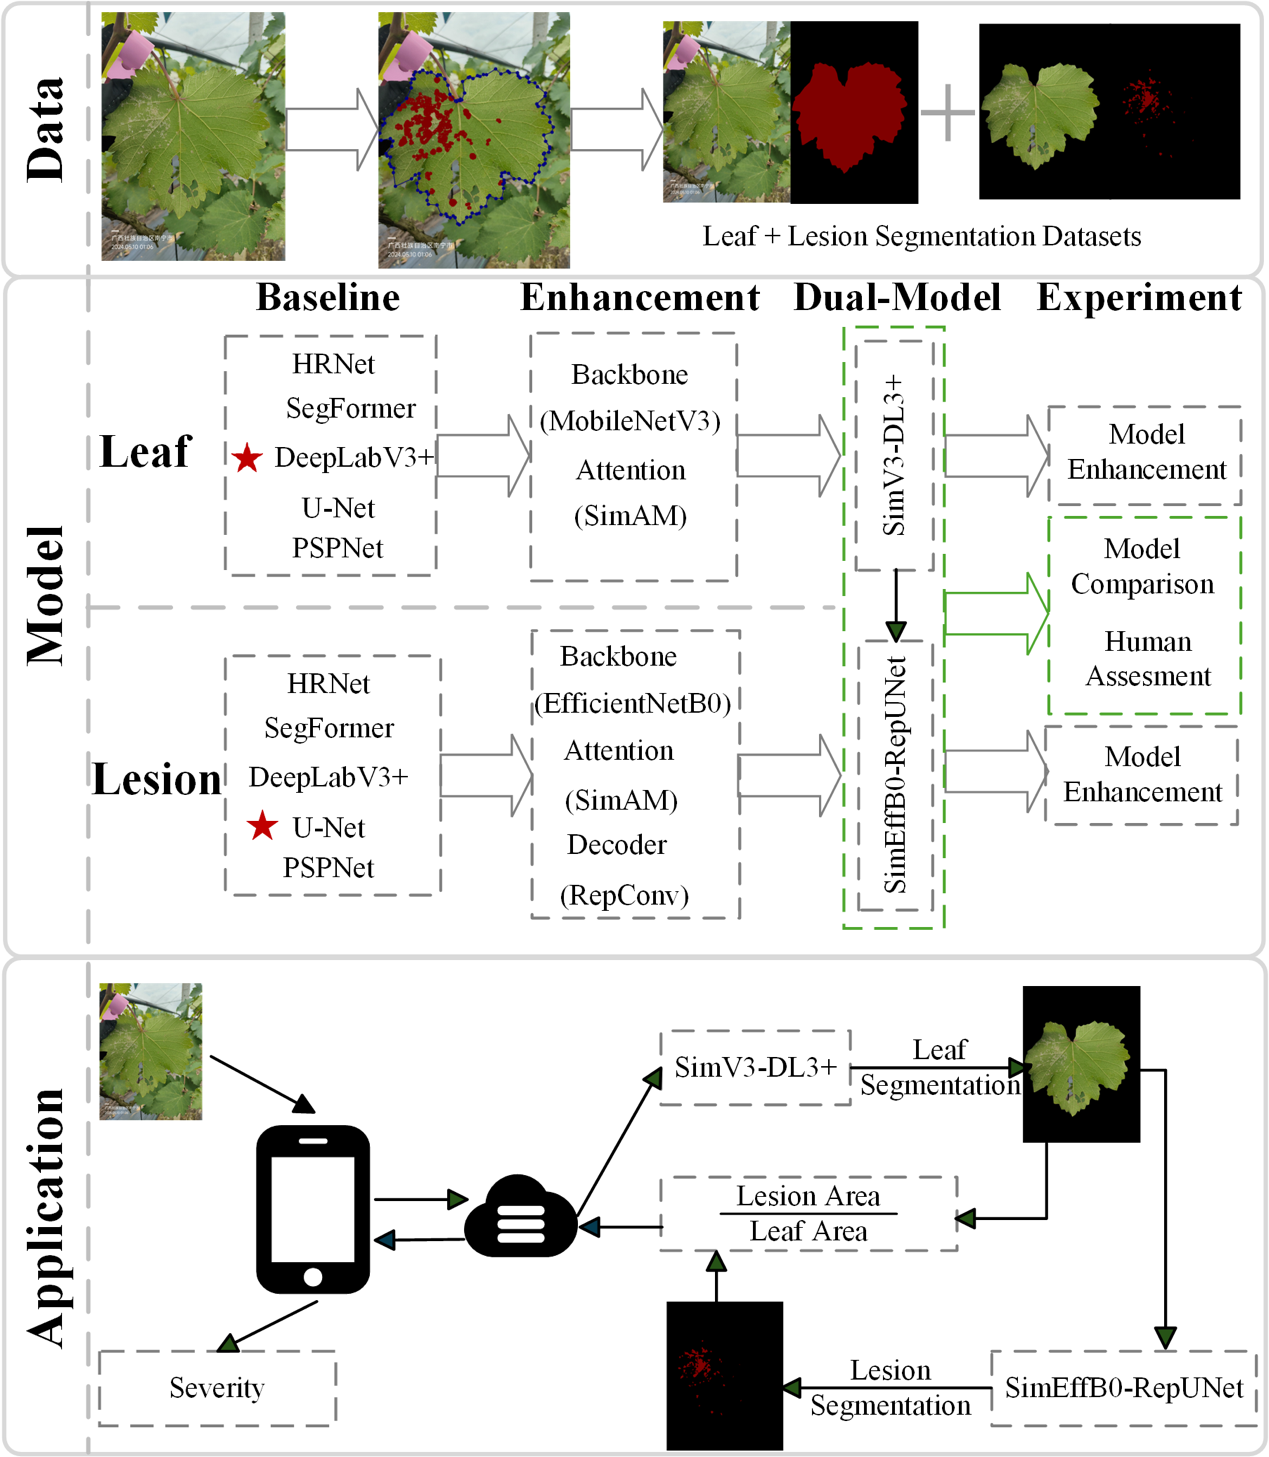
\includegraphics[width=\linewidth]{DSLL-Net-media/media/image1.png}

\hypertarget{fig:1}{}Fig. 1. Overall workflow of data preparation, dual-stage model
development, and mobile application deployment.

\hypertarget{data-preparation}{%
\subsection{Data Preparation}\label{data-preparation}}

A total of 696 field images were collected between April and August 2024
at Mingyang and Du'an in Guangxi, China. Images were captured using a
Huawei P70 and an iPhone 15 at a distance of 15--20 cm, with each image
focused on a single leaf. Images with clear leaf structures, appropriate
viewing angles, and no severe occlusion were retained.

The collection period covered different stages of disease occurrence in
field conditions, allowing the dataset to include leaves with mild,
moderate, and relatively severe symptoms. Images affected by strong
direct sunlight, severe blur, or incomplete leaf visibility were excluded
to reduce annotation ambiguity. This filtering was intended to maintain
reliable pixel-level labels while still preserving typical background
variation encountered in vineyard scenes.

Leaf and lesion regions were manually annotated using LabelMe (v3.16.7),
generating binary masks for leaf/background and lesion/non-lesion
classes. These annotations were used to construct three datasets for
leaf segmentation, lesion segmentation, and single-stage lesion
segmentation, as summarized in Table 1.

Table. 1 An overview of the constructed datasets and their corresponding
modeling tasks.

\scriptsize
\setlength{\tabcolsep}{2pt}
\begin{longtable}[]{@{}>{\raggedright\arraybackslash}p{0.13\linewidth}>{\raggedright\arraybackslash}p{0.15\linewidth}>{\raggedright\arraybackslash}p{0.13\linewidth}>{\raggedright\arraybackslash}p{0.17\linewidth}>{\raggedright\arraybackslash}p{0.17\linewidth}>{\raggedright\arraybackslash}p{0.16\linewidth}@{}}
\toprule
Dataset & Input to model & Label(s) & Construction & Task & Models using it \\
\midrule
\endhead
Leaf segmentation & Original full RGB field image & Leaf mask (binary) &
Manual annotation on original image & Leaf extraction from background &
Stage-1 models: DeepLabV3+ baseline comparisons and SimV3-DL3+ \\
Lesion segmentation & Cropped leaf ROI & Lesion mask (binary, cropped
consistently) & Crop leaf regions using leaf masks; pair with cropped
lesion masks & Fine-grained lesion segmentation within leaf & Stage-2
models: U-Net family and SimEffB0-RepUNet \\
Single-stage segmentation & Original full RGB field image & Lesion mask
(binary) & Original images + lesion masks & Single-stage lesion
segmentation & Single-stage baselines: U-Net, DeepLabV3+, PSPNet, HRNet,
and SegFormer \\
\bottomrule
\end{longtable}
\setlength{\tabcolsep}{6pt}
\normalsize

All datasets used the same train--test split: 567 images for training
and 129 for testing. To match deployment conditions, the second-stage
lesion model used leaf regions predicted by the first-stage model rather
than ground-truth leaf masks.

This setting is important because the lesion stage receives imperfect
leaf regions during real use. Evaluating the full pipeline with predicted
leaf masks therefore provides a more realistic estimate of deployment
performance than testing lesion segmentation only on manually cropped
ground-truth leaf regions. The single-stage dataset was retained as a
direct comparison to quantify the benefit of explicitly separating leaf
and lesion segmentation.

\hypertarget{dual-stage-segmentation-model}{%
\subsection{Dual-Stage Segmentation
Model}\label{dual-stage-segmentation-model}}

\hypertarget{leaf-segmentation-model-simv3-dl3}{%
\subsection{Leaf Segmentation Model
SimV3-DL3+}\label{leaf-segmentation-model-simv3-dl3}}

The first stage aims to segment leaf regions accurately while keeping the
model compact for mobile deployment. Five representative segmentation
models (DeepLabV3+ \textcolor{blue}{\hyperlink{ref:20}{[20]}}, U-Net
\textcolor{blue}{\hyperlink{ref:24}{[24]}}, PSPNet
\textcolor{blue}{\hyperlink{ref:25}{[25]}}, SegFormer
\textcolor{blue}{\hyperlink{ref:26}{[26]}}, and HRNet
\textcolor{blue}{\hyperlink{ref:27}{[27]}}) were evaluated, and
DeepLabV3+ was selected as the baseline because it provided the best
accuracy with moderate complexity. To improve efficiency, MobileNetV3
\textcolor{blue}{\hyperlink{ref:21}{[21]}} was used as the backbone. Its
original SE module was replaced with SimAM, which enhances spatial
responses without adding learnable parameters.
The resulting SimV3-DL3+ model is shown in \hyperlink{fig:2}{\textcolor{blue}{Fig. 2}}.

The choice of DeepLabV3+ is based on its atrous spatial pyramid pooling,
which captures multi-scale context useful for separating complete leaf
regions from heterogeneous backgrounds. MobileNetV3 was selected because
it offers a stronger accuracy--efficiency balance than MobileNetV2
\textcolor{blue}{\hyperlink{ref:28}{[28]}} and a more compact alternative
than MobileNetV4 \textcolor{blue}{\hyperlink{ref:29}{[29]}} in this task.
Replacing SE \textcolor{blue}{\hyperlink{ref:30}{[30]}} with SimAM
\textcolor{blue}{\hyperlink{ref:31}{[31]}} was intended to strengthen
spatial attention for boundary pixels and reduce the parameter cost
introduced by channel attention.

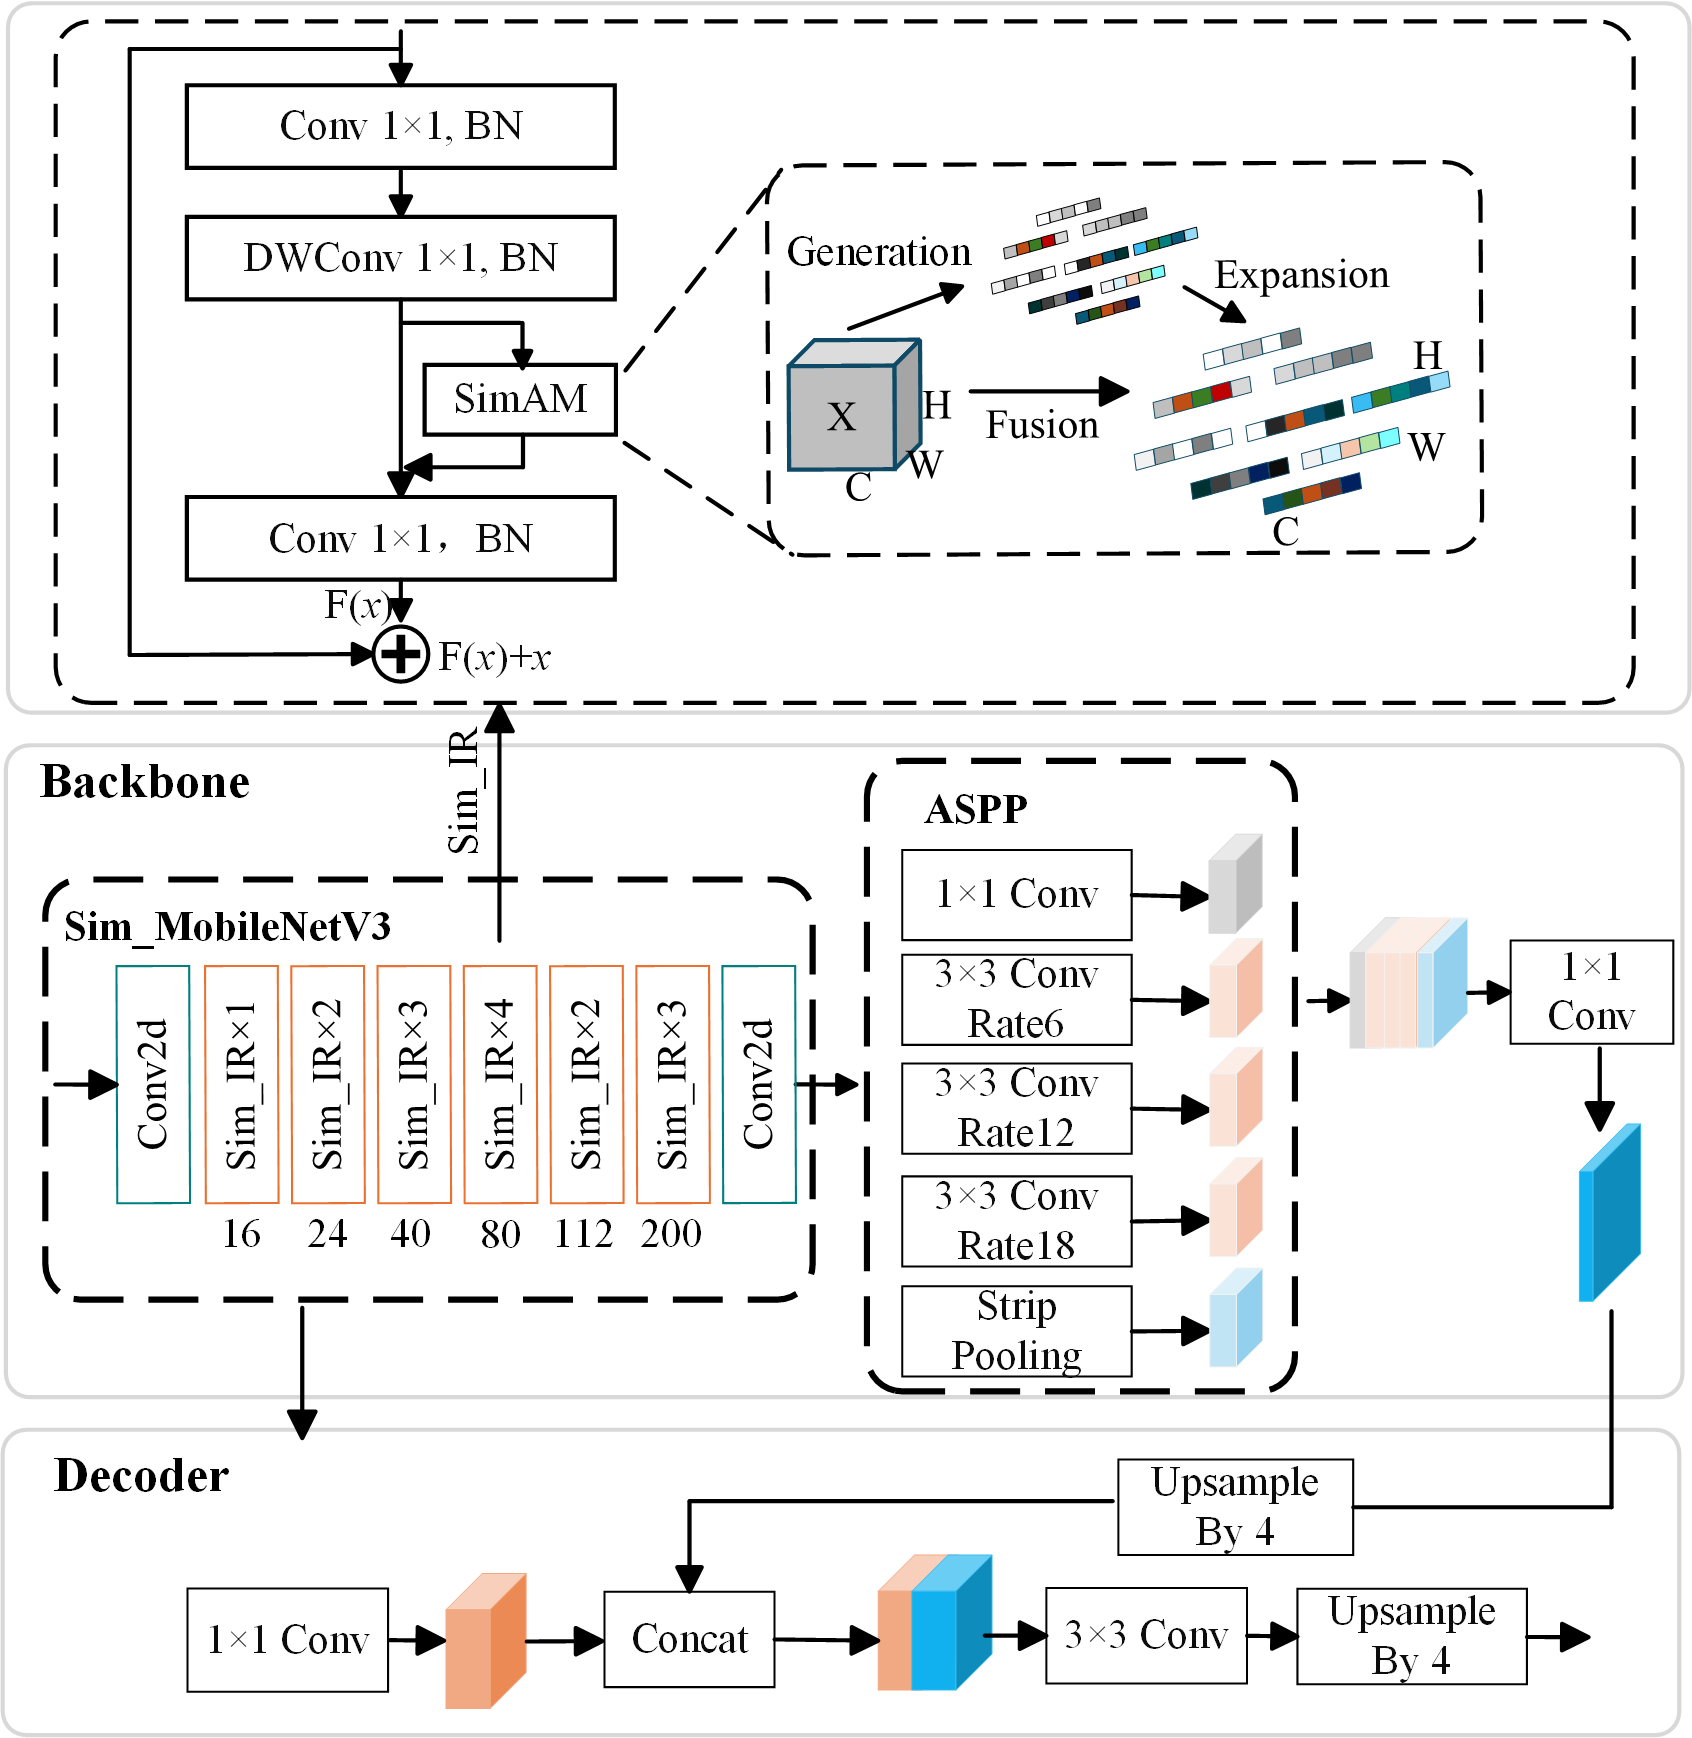
\includegraphics[width=\linewidth]{DSLL-Net-media/media/image2.png}

\hypertarget{fig:2}{}Fig. 2. Architecture of the SimV3-DL3+ model. Sim\_IR denotes the
InvertedResidual block enhanced with SimAM attention.

\hypertarget{lesion-segmentation-model-simeffb0-repunet}{%
\subsection{\texorpdfstring{Lesion Segmentation Model (SimEffB0-RepUNet)
}{Lesion Segmentation Model (SimEffB0-RepUNet) }}\label{lesion-segmentation-model-simeffb0-repunet}}

The second stage focuses on small and irregular lesion regions, where
boundary precision is more difficult than leaf extraction. U-Net was
selected as the baseline after comparison with DeepLabV3+, PSPNet,
SegFormer, and HRNet. To reduce the parameter cost of the conventional
VGG16 encoder, EfficientNet-B0 was adopted as the encoder. Its SE module
was replaced with SimAM to improve spatial lesion representation without
increasing model complexity. RepConv blocks were further introduced in
the decoder to strengthen feature fusion and boundary reconstruction
during training while preserving efficient inference after
re-parameterization \textcolor{blue}{\hyperlink{ref:23}{[23]}}. The final model, SimEffB0-RepUNet, is shown in
\hyperlink{fig:3}{\textcolor{blue}{Fig. 3}}.

This design follows the different requirements of lesion segmentation.
EfficientNet-B0 provides compact multi-scale feature extraction for
fine-grained lesion patterns, SimAM increases sensitivity to spatially
sparse symptoms, and RepConv improves decoder representation during
training through multi-branch convolution. After re-parameterization,
RepConv is converted into a single convolutional structure, so the
decoder gains training-time representation capacity without increasing
inference complexity.

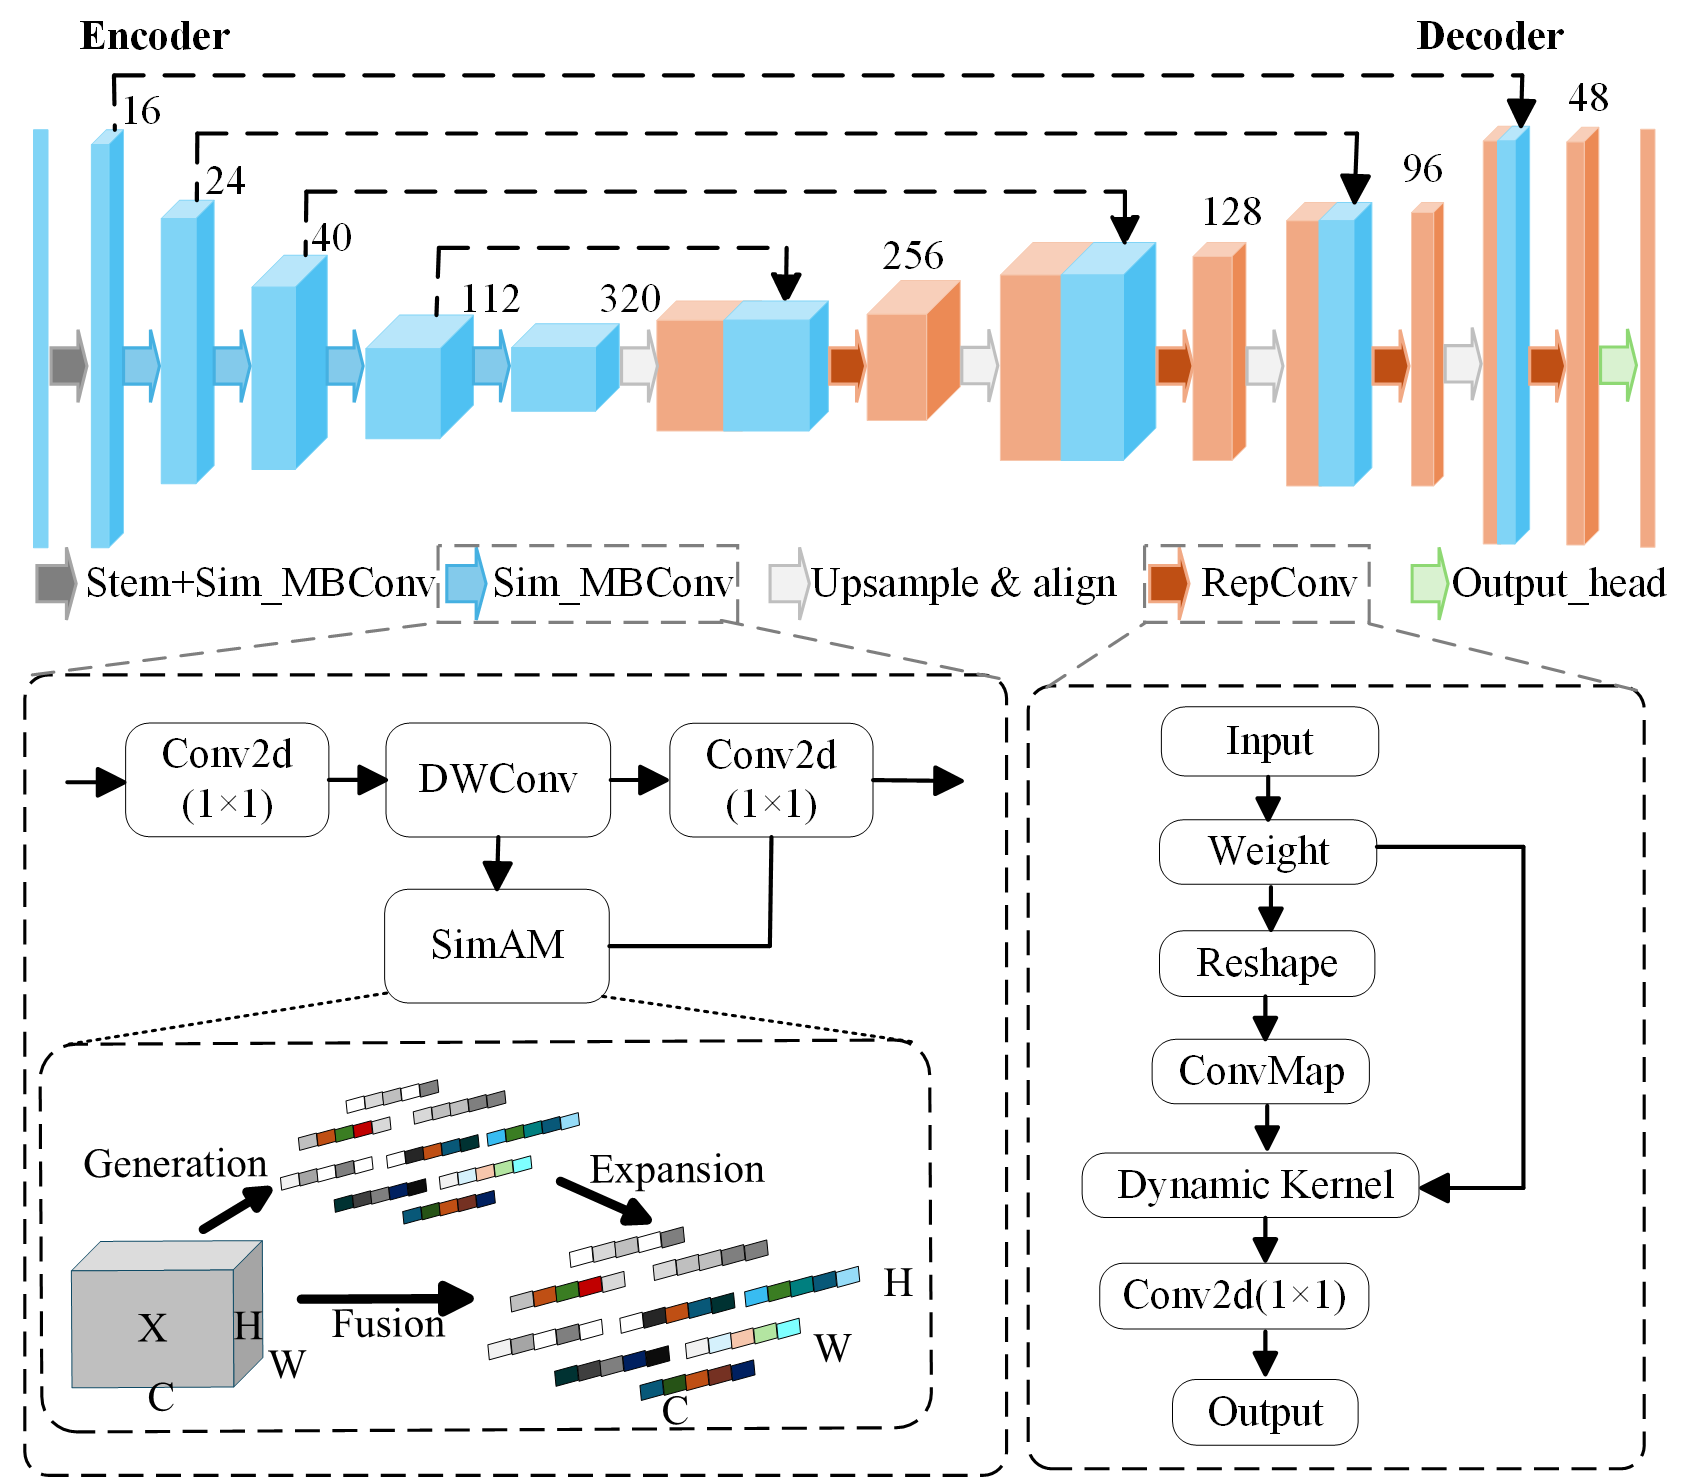
\includegraphics[width=\linewidth]{DSLL-Net-media/media/image3.png}

\hypertarget{fig:3}{}Fig. 3. Architecture of SimEffB0-RepUNet, which uses a SimAM-enhanced
EfficientNet-B0 encoder and RepConv modules in the decoder.

\hypertarget{experimental-design}{%
\subsection{Experimental design}\label{experimental-design}}

\hypertarget{leaf-segmentation}{%
\subsection{Leaf segmentation}\label{leaf-segmentation}}

For leaf segmentation, U-Net, DeepLabV3+, PSPNet, HRNet, and SegFormer
were compared using mPA, IoU-Background, IoU-Leaf, mIoU, parameter count,
and inference time. IoU-Leaf was treated as the primary metric. Backbone
selection was then evaluated within DeepLabV3+ using MobileNetV2,
MobileNetV3, MobileNetV4 \textcolor{blue}{\hyperlink{ref:29}{[29]}},
StarNetS1 \textcolor{blue}{\hyperlink{ref:32}{[32]}}, and
EfficientNet-B0. Finally,
MobileNetV3 with SE attention was compared with the SimAM-enhanced
variant to assess the contribution of parameter-free spatial attention
\textcolor{blue}{\hyperlink{ref:30}{[30]}, \hyperlink{ref:31}{[31]}}.

The experimental sequence was designed to avoid changing multiple
factors simultaneously. First, the baseline segmentation architecture was
selected. Then, lightweight backbones were compared under the same
DeepLabV3+ framework. Finally, the attention module was changed while
keeping the selected architecture fixed, allowing the contribution of
SimAM to be isolated.

\hypertarget{lesion-segmentation}{%
\subsection{Lesion segmentation}\label{lesion-segmentation}}

For lesion segmentation, candidate architectures were first compared to
select the baseline, followed by ablation experiments on backbone,
attention module, and decoder convolution. The evaluated backbones
included VGG16, ResNet50 \textcolor{blue}{\hyperlink{ref:27}{[27]}},
ResNetRS50 \textcolor{blue}{\hyperlink{ref:33}{[33]}}, MobileNetV2,
MobileNetV3, and
EfficientNet-B0. The attention comparison included SE, ECA, CBAM, and
SimAM, and the decoder comparison included Conv, Conv×2, RepConv, ODConv,
PConv, and CondConv2D \textcolor{blue}{\hyperlink{ref:34}{[34}-\hyperlink{ref:38}{38]}}.
IoU-Disease was the primary metric, together with
mPA, IoU-Background, mIoU, parameter count, and inference time.

Because lesion pixels occupy a smaller proportion of the image than leaf
pixels, IoU-Disease was emphasized over global accuracy. Parameter count
and inference time were reported together with segmentation metrics to
ensure that improvements were not obtained solely by increasing model
size. This is particularly relevant for mobile or edge deployment, where
small increases in latency can affect usability in field surveys.

\hypertarget{model-comparison-experiments}{%
\subsection{Model Comparison
Experiments}\label{model-comparison-experiments}}

To evaluate the dual-stage strategy, five single-stage models were
compared with a conventional DeepLabV3+ + U-Net pipeline and the proposed
SimV3-DL3+ + SimEffB0-RepUNet pipeline. Performance was measured by
IoU-Leaf, IoU-Disease, parameter count, and average inference time per
image. For dual-stage models, inference time included both segmentation
stages and intermediate processing.

The comparison was intended to answer two questions. First, it tested
whether lesion segmentation from full field images can match a pipeline
that explicitly extracts the leaf region before lesion detection.
Second, it evaluated whether the proposed lightweight modifications can
improve the conventional dual-stage configuration without increasing
model size. This setting directly reflects the severity estimation task,
because the final value depends on both the numerator (lesion area) and
the denominator (leaf area).

\hypertarget{expert-visual-evaluation-and-model-prediction}{%
\subsection{Expert Visual Evaluation and Model
Prediction}\label{expert-visual-evaluation-and-model-prediction}}

To compare automated severity estimation with human judgment, 15 trained
technicians visually estimated disease severity on representative leaf
images. Their assessments were compared with model predictions for the
same images.

\hypertarget{experimental-setup}{%
\subsection{Experimental setup}\label{experimental-setup}}

Experiments were conducted on an NVIDIA GeForce RTX 4060 Ti GPU with an
Intel Core i5-13490F CPU and 32 GB RAM. Models were trained in Python 3.8
with CUDA 11.8 using Adam, a batch size of 2, an initial learning rate of
\(1 \times 10^{-5}\), cosine annealing to \(1 \times 10^{-6}\), and 500
epochs. All images were resized to \(512 \times 512\). Dice loss was used:

All models in the same comparison group were trained under the same
input resolution, optimization settings, and train--test split. This
ensured that differences in performance mainly reflected architectural
design rather than data partitioning or training protocol. Inference time
was measured on the test set and averaged per image. For the proposed
pipeline, the reported time includes leaf prediction, cropping or
intermediate processing, lesion prediction, and pixel counting for
severity calculation.

\begin{equation}
\mathcal{L}_{D\text{ice}} = 1 - \frac{2|X \cap Y|}{\left| X \right| + |Y|}
\tag{1}
\end{equation}

where \(X\) and \(Y\) denote the predicted and ground-truth masks.

\hypertarget{evaluation-metrics}{%
\subsection{Evaluation metrics}\label{evaluation-metrics}}

Segmentation performance was evaluated using PA, mPA, IoU, and mIoU:

\begin{equation}
PA = \frac{\sum_{i = 0}^{k}P_{\text{ii}}}{\sum_{i = 0}^{k}{\sum_{j = 0}^{k}P_{\text{ij}}}}
\tag{2}
\end{equation}

where \(P_{\text{ii}}\) denotes correctly classified pixels of class
\(i\), and \(P_{\text{ij}}\) denotes pixels whose ground-truth class is
\(i\) but are predicted as class \(j\).

\begin{equation}
\text{mPA} = \frac{1}{K + 1}\sum_{i = 0}^{K}\frac{P_{\text{ii}}}{\sum_{j = 0}^{K} P_{\text{ij}}}
\tag{3}
\end{equation}

Here, \(K+1\) is the number of classes including background.

\begin{equation}
\text{IoU}_{i} = \frac{TP_{i}}{TP_{i} + FP_{i} + FN_{i}}
\tag{4}
\end{equation}

where \(TP_{i}\), \(FP_{i}\), and \(FN_{i}\) are true-positive,
false-positive, and false-negative pixels for class \(i\).

\begin{equation}
\text{mIoU} = \frac{1}{K + 1}\sum_{i = 0}^{K}\text{IoU}_{i}
= \frac{1}{K + 1}\sum_{i = 0}^{K}\frac{TP_{i}}{TP_{i} + FP_{i} + FN_{i}}
\tag{5}
\end{equation}

Severity estimation was evaluated using \(R^{2}\), MAE, and RMSE:

After segmentation, disease severity was computed as:

\begin{equation}
S = \frac{A_{\text{lesion}}}{A_{\text{leaf}}}
\tag{9}
\end{equation}

where \(A_{\text{lesion}}\) and \(A_{\text{leaf}}\) are the pixel areas
of the predicted lesion and leaf masks, respectively. This formulation
directly links segmentation performance to the final agronomic severity
indicator.

\begin{equation}
R^{2} = 1 - \frac{\sum_{i = 1}^{n}\left( y_{i} - {\widetilde{y}}_{i} \right)^{2}}{\sum_{i = 1}^{n}\left( y_{i} - \bar{y} \right)^{2}}
\tag{6}
\end{equation}

where \(n\) is the number of samples, \(y_{i}\) and
\({\widetilde{y}}_{i}\) are the actual and predicted values, and
\(\bar{y}\) is the mean of all actual values.

\begin{equation}
\text{MAE} = \frac{1}{n}\sum_{i = 1}^{n}{|y_{i} - {\widetilde{y}}_{i}|}
\tag{7}
\end{equation}


\begin{equation}
\text{RMSE} = \sqrt{\frac{1}{n}\sum_{i = 1}^{n}{(y_{i} - {\widetilde{y}}_{i})}^{2}}
\tag{8}
\end{equation}

\hypertarget{results}{%
\section{Results}\label{results}}

\hypertarget{leaf-segmentation-1}{%
\subsection{Leaf segmentation}\label{leaf-segmentation-1}}

Among the five leaf segmentation models (\hyperlink{fig:4}{\textcolor{blue}{Fig. 4}}), DeepLabV3+ achieved
the best overall accuracy, with an mPA of 99.11\%, IoU-Background of
98.70\%, IoU-Leaf of 97.49\%, and mIoU of 98.09\%. It also maintained
moderate model size and inference time, and was therefore selected as the
baseline for leaf segmentation.

Although HRNet also produced competitive accuracy, its larger model size
and longer inference time were less suitable for the intended deployment
scenario. U-Net ranked behind DeepLabV3+ in accuracy and required more
parameters, whereas PSPNet and SegFormer provided lower segmentation
accuracy despite their compactness. These results indicate that
DeepLabV3+ provides the best starting point for stage-1 leaf extraction.

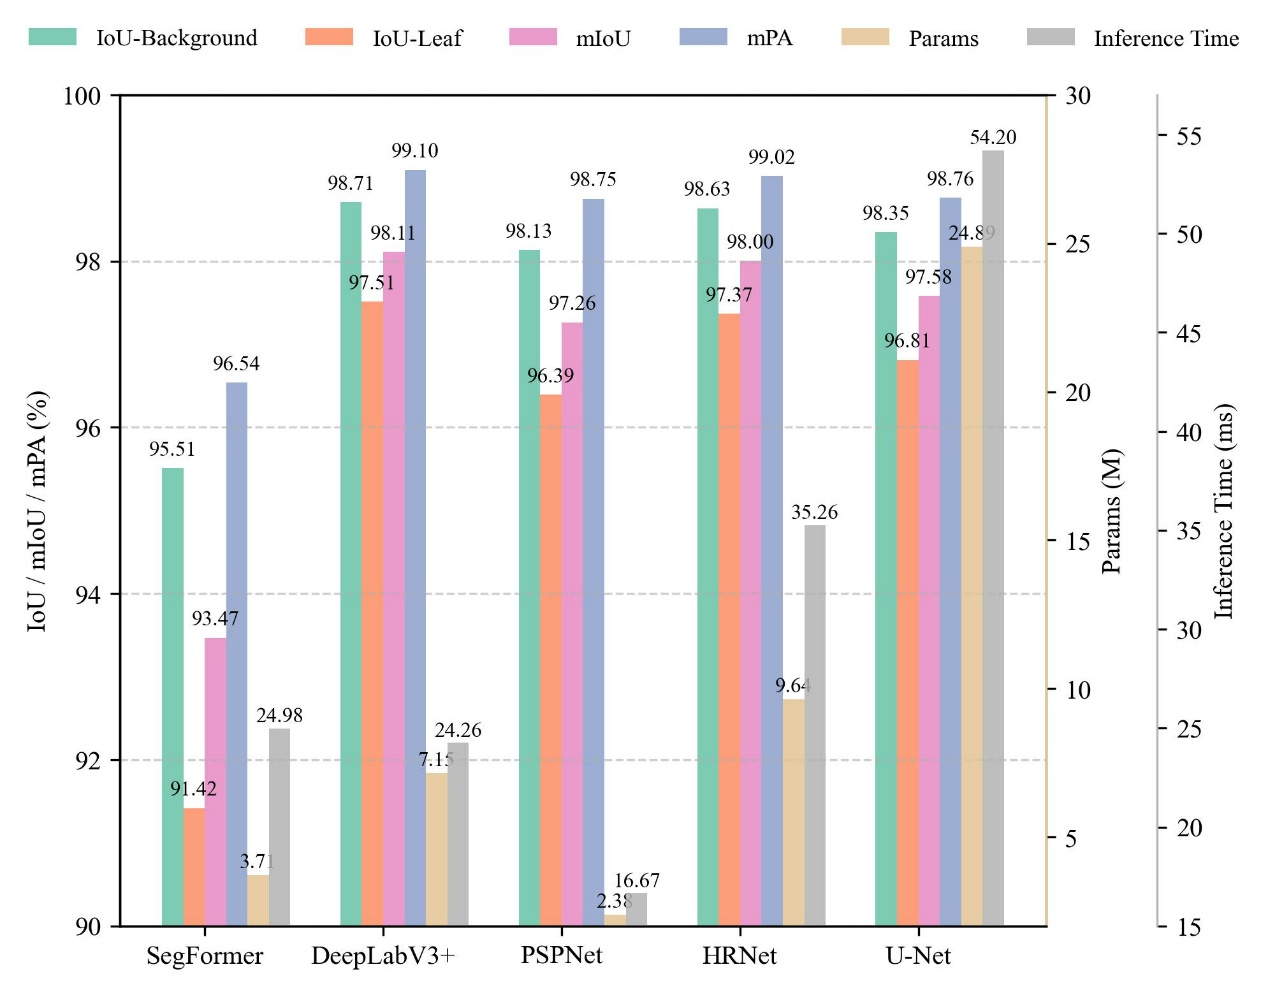
\includegraphics[width=\linewidth]{DSLL-Net-media/media/image4.jpeg}

\hypertarget{fig:4}{}Fig. 4. Leaf segmentation comparison of SegFormer, DeepLabV3+, PSPNet,
HRNet, and U-Net.

Backbone comparison further showed that Sim\_MobileNetV3 provided the
best accuracy--efficiency balance (\hyperlink{fig:5}{\textcolor{blue}{Fig. 5}}), reaching the highest mPA
(99.19\%) and mIoU (98.30\%) with only 4.83 M parameters and 20.62 ms
inference time.

Compared with the MobileNetV2 baseline, Sim\_MobileNetV3 improved
accuracy while reducing parameter count. EfficientNet-B0 achieved
comparable accuracy but required more parameters and longer inference,
and MobileNetV4 did not provide a favorable trade-off in this dataset.
The improvement obtained by Sim\_MobileNetV3 supports the use of
parameter-free spatial attention for leaf boundary extraction.
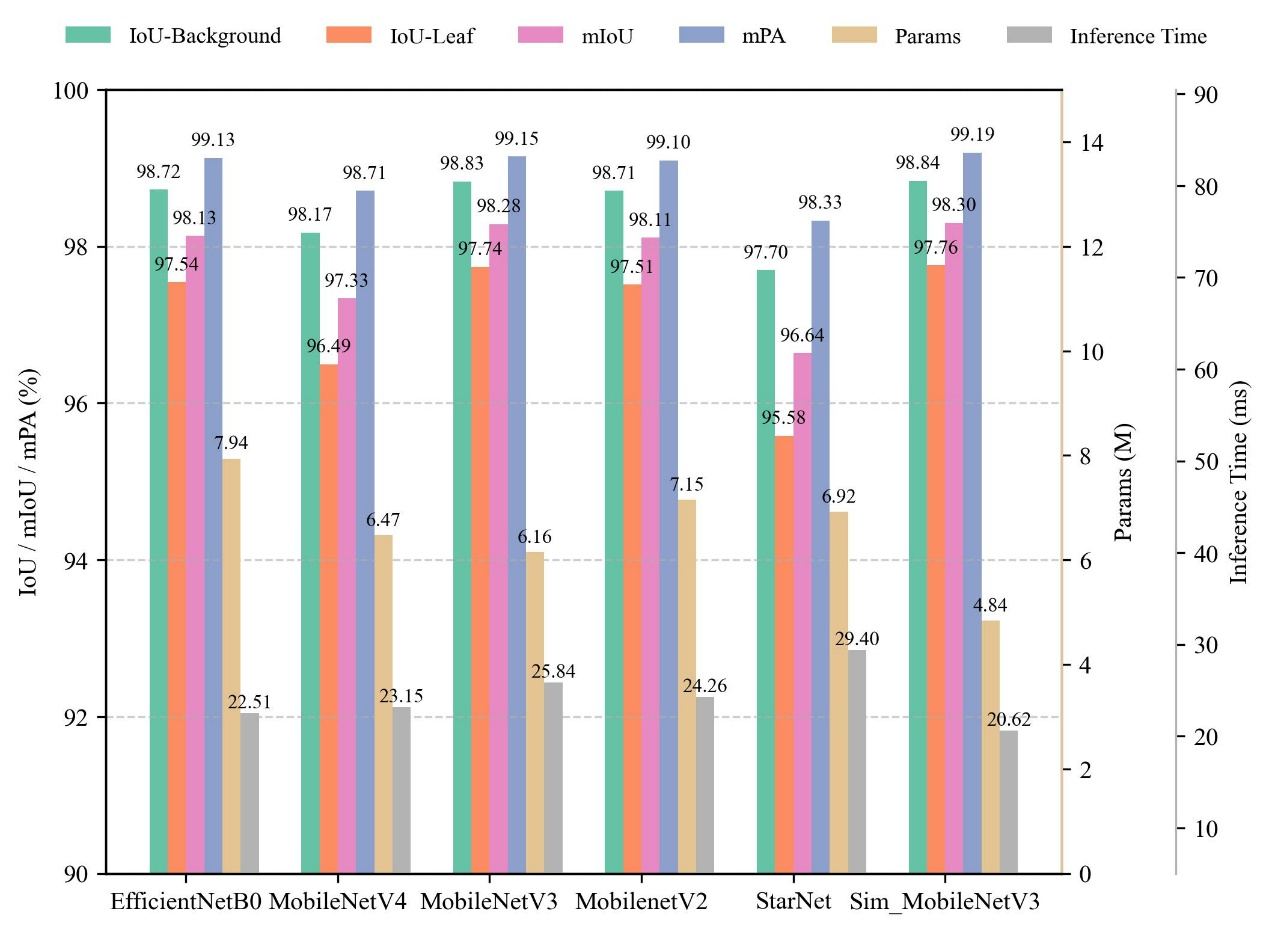
\includegraphics[width=\linewidth]{DSLL-Net-media/media/image5.jpeg}

\hypertarget{fig:5}{}Fig. 5. Leaf segmentation performance of DeepLabV3+ with different
backbones.

\hypertarget{lesion-segmentation-1}{%
\subsection{Lesion segmentation}\label{lesion-segmentation-1}}

For lesion segmentation, U-Net achieved the highest accuracy among the
candidate architectures (\hyperlink{fig:6}{\textcolor{blue}{Fig. 6}}), with an mIoU of 84.97\% and
IoU-Disease of 73.07\%. Although it had the largest parameter count
(24.89 M) and longest inference time (51.53 ms), its accuracy made it the
baseline for subsequent optimization.

HRNet and DeepLabV3+ showed competitive lesion segmentation performance,
but neither exceeded U-Net in IoU-Disease. PSPNet was the most efficient
but had substantially lower lesion accuracy, indicating that speed alone
is insufficient for reliable severity estimation. The strong performance
of U-Net confirmed the value of encoder--decoder feature fusion for
small lesion delineation.

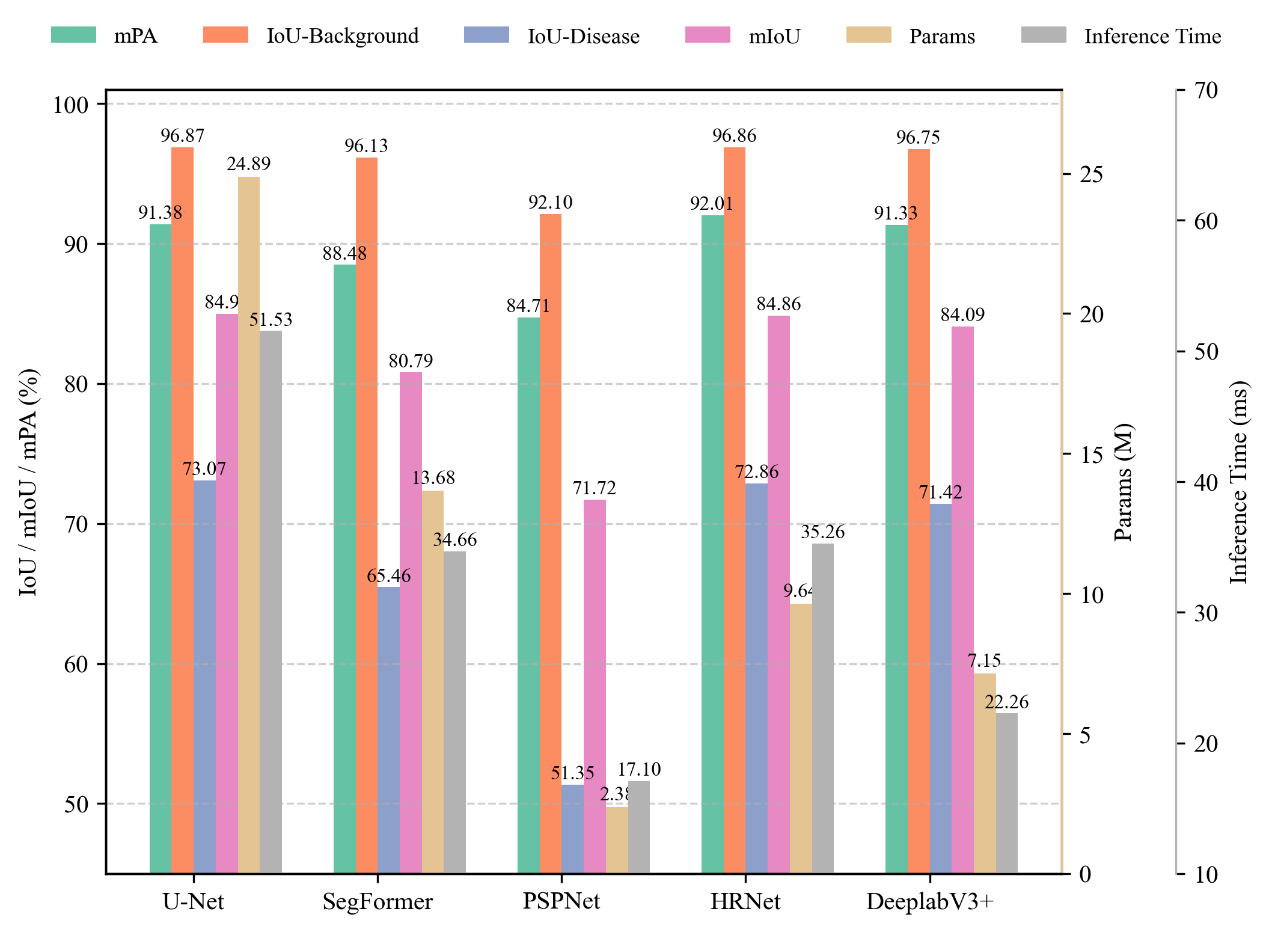
\includegraphics[width=\linewidth]{DSLL-Net-media/media/image6.png}

\hypertarget{fig:6}{}Fig. 6. Lesion segmentation comparison of U-Net, SegFormer, PSPNet,
HRNet, and DeepLabV3+.

Backbone evaluation showed that EfficientNet-B0 achieved the best
balance for lesion segmentation (\hyperlink{fig:7}{\textcolor{blue}{Fig. 7}}), providing the highest mIoU and
IoU-Disease while reducing parameters by more than 82\% compared with
ResNet50 and achieving the fastest inference time (25.01 ms).

This result suggests that EfficientNet-B0 is better suited to the lesion
stage than heavier residual backbones. ResNet50 and ResNetRS50 produced
similar accuracy but with much larger parameter counts, while the
MobileNet variants were efficient but less accurate. EfficientNet-B0 was
therefore adopted as the encoder for the final lesion model.

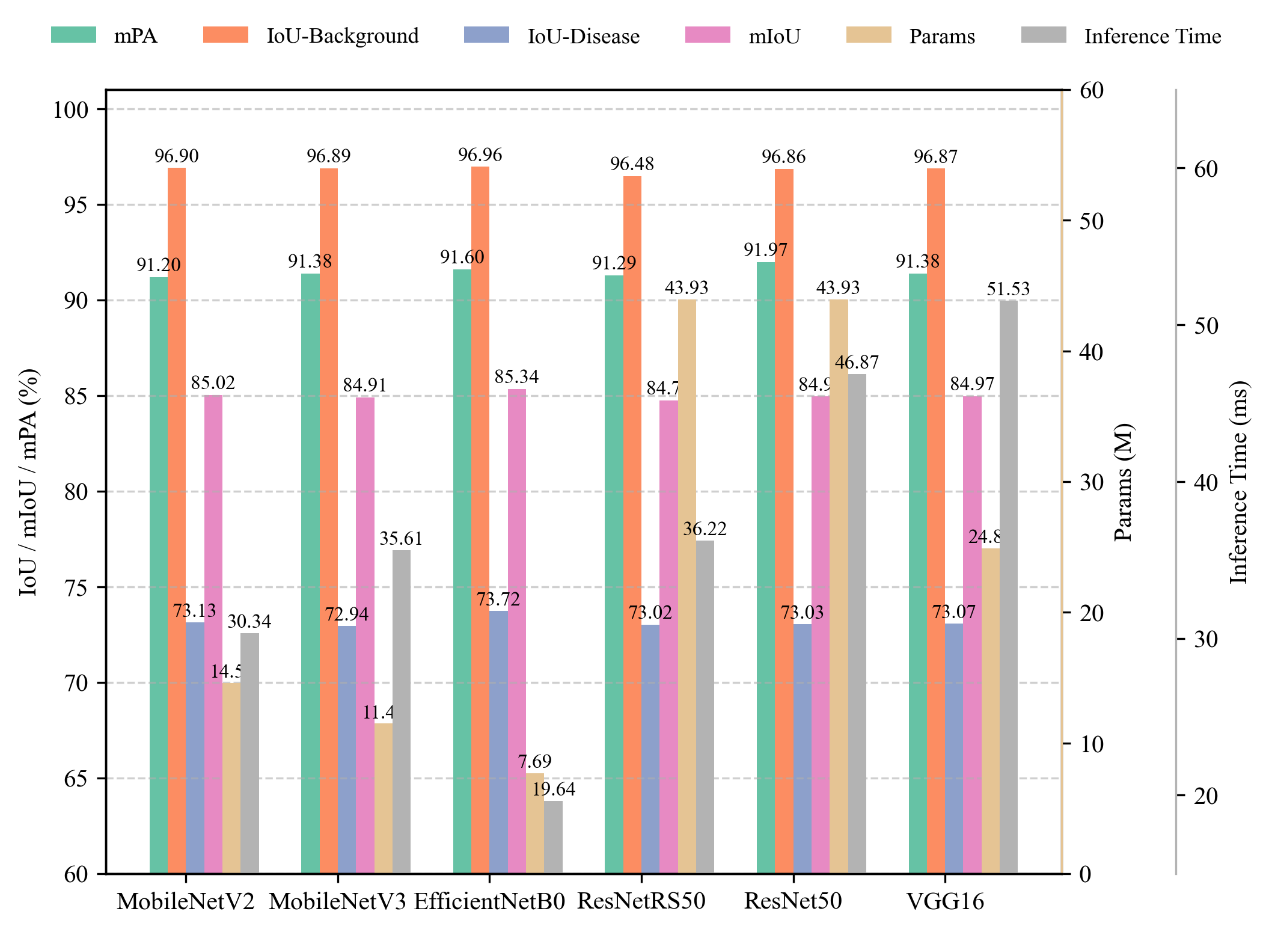
\includegraphics[width=\linewidth]{DSLL-Net-media/media/image7.png}

\hypertarget{fig:7}{}Fig. 7. Lesion segmentation performance of U-Net with different
backbones.

Attention comparison indicated that SimAM improved mIoU (85.46\%) and
IoU-Disease (73.94\%) over SE while reducing the parameter count to 7.05
M (\hyperlink{fig:8}{\textcolor{blue}{Fig. 8}}). It therefore provided the most favorable trade-off among the
evaluated attention modules.

ECA and CBAM provided limited or inconsistent gains and increased
latency. The advantage of SimAM is that it improves spatial sensitivity
without introducing additional learnable parameters, which is beneficial
for small and irregular disease lesions.

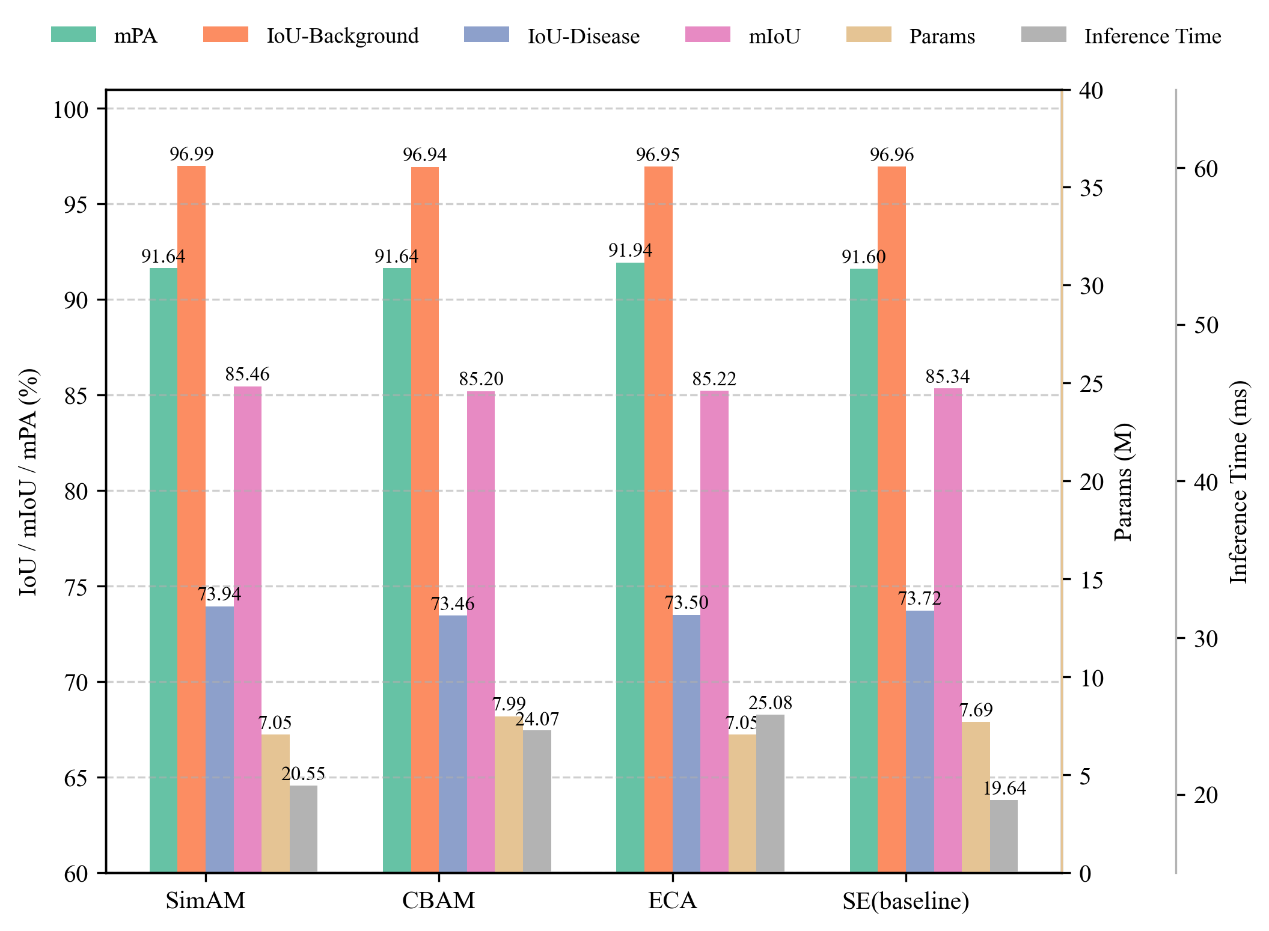
\includegraphics[width=\linewidth]{DSLL-Net-media/media/image8.png}

\hypertarget{fig:8}{}Fig. 8. Lesion segmentation performance with different attention modules.

Among decoder variants, RepConv achieved the best overall performance
(\hyperlink{fig:9}{\textcolor{blue}{Fig. 9}}), with the highest IoU-Disease (74.30\%) and mIoU (85.64\%), a
moderate parameter count (7.73 M), and the shortest inference time
(17.33 ms). RepConv was therefore adopted in the final lesion model.

The comparison indicates that the decoder plays a critical role in
recovering fine lesion boundaries. CondConv2D achieved competitive
accuracy but required more parameters, whereas ODConv increased
computational cost without improving accuracy. RepConv provided the best
combination of boundary accuracy and inference efficiency.

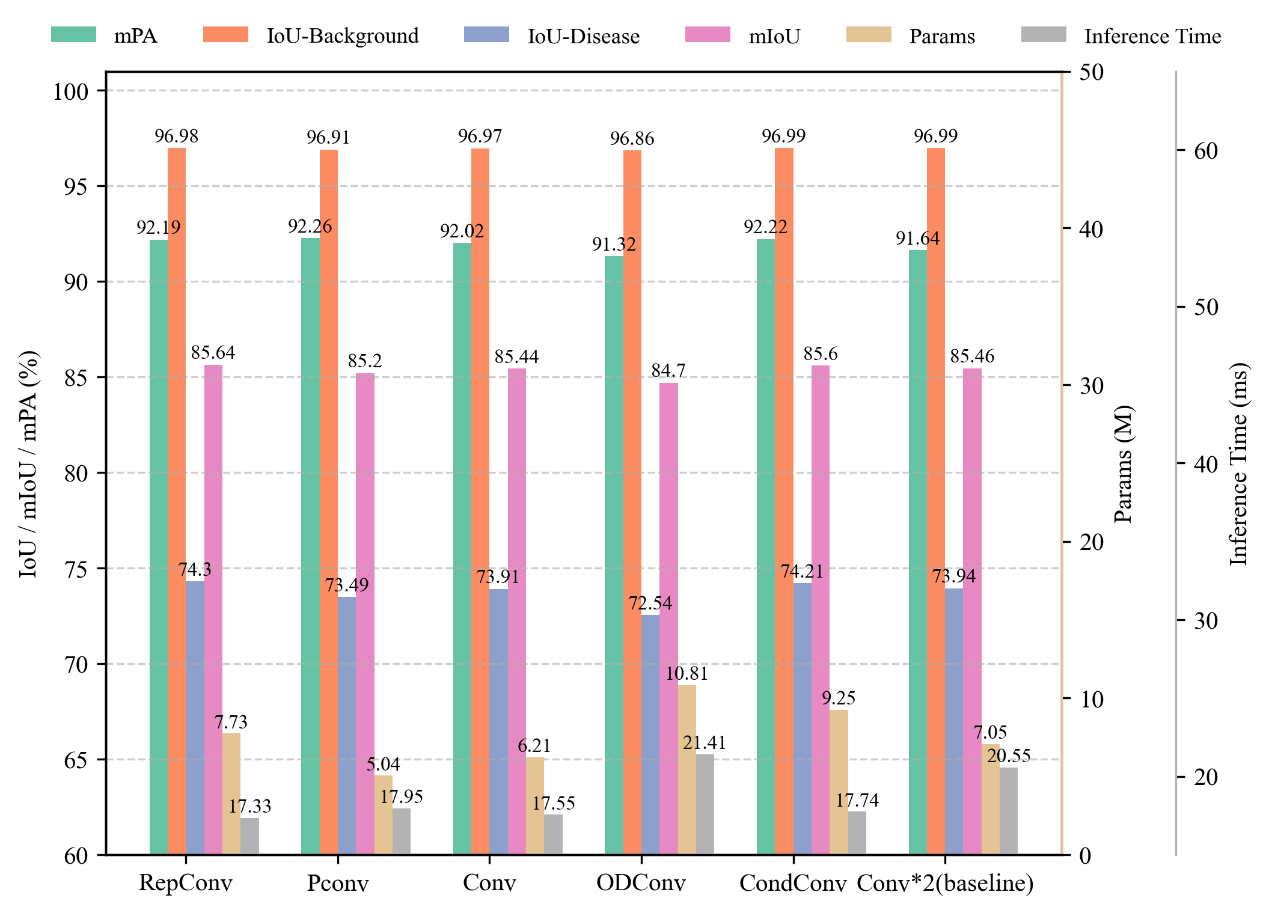
\includegraphics[width=\linewidth]{DSLL-Net-media/media/image9.png}

\hypertarget{fig:9}{}Fig. 9. Lesion segmentation performance with different decoder
convolution variants.

Severity estimation based on SimEffB0-RepUNet outputs strongly agreed
with ground truth (\hyperlink{fig:S1}{\textcolor{blue}{Fig. S1}}), achieving \(R^{2}=0.976\), MAE = 0.012, and
RMSE = 0.019 on the test set.

The low MAE and RMSE indicate that the proposed method not only ranks
samples consistently with the reference values but also produces
numerically close severity estimates. This is important for practical
applications such as fungicide evaluation and disease progression
monitoring, where small differences in lesion coverage may influence
management decisions. The high \(R^{2}\) further suggests that the
segmentation-derived severity values capture most of the variation in
the reference measurements.

\hypertarget{model-comparison}{%
\subsection{Model comparison}\label{model-comparison}}

The proposed dual-stage model outperformed both single-stage models and
the conventional dual-stage baseline (\hyperlink{fig:10}{\textcolor{blue}{Fig. 10}}). It achieved 97.76\%
IoU-Leaf and 74.30\% IoU-Disease with 12.56 M parameters and 2261 ms
inference time. In comparison, DeepLabV3+ + U-Net reached 97.49\%
IoU-Leaf and 72.71\% IoU-Disease with 32.04 M parameters and 2303 ms
inference time. Qualitative results (\hyperlink{fig:S2}{\textcolor{blue}{Fig. S2}}) further showed that the
proposed model reduced leaf over-segmentation and improved lesion
boundary delineation.

Among single-stage models, DeepLabV3+ and U-Net achieved the strongest
lesion results, but both were less accurate than the dual-stage
pipelines. This confirms that direct lesion segmentation from full field
images is affected by background and leaf boundary interference. The
proposed model improves both accuracy and compactness relative to the
conventional dual-stage baseline, showing that task decomposition should
be paired with stage-specific lightweight design.

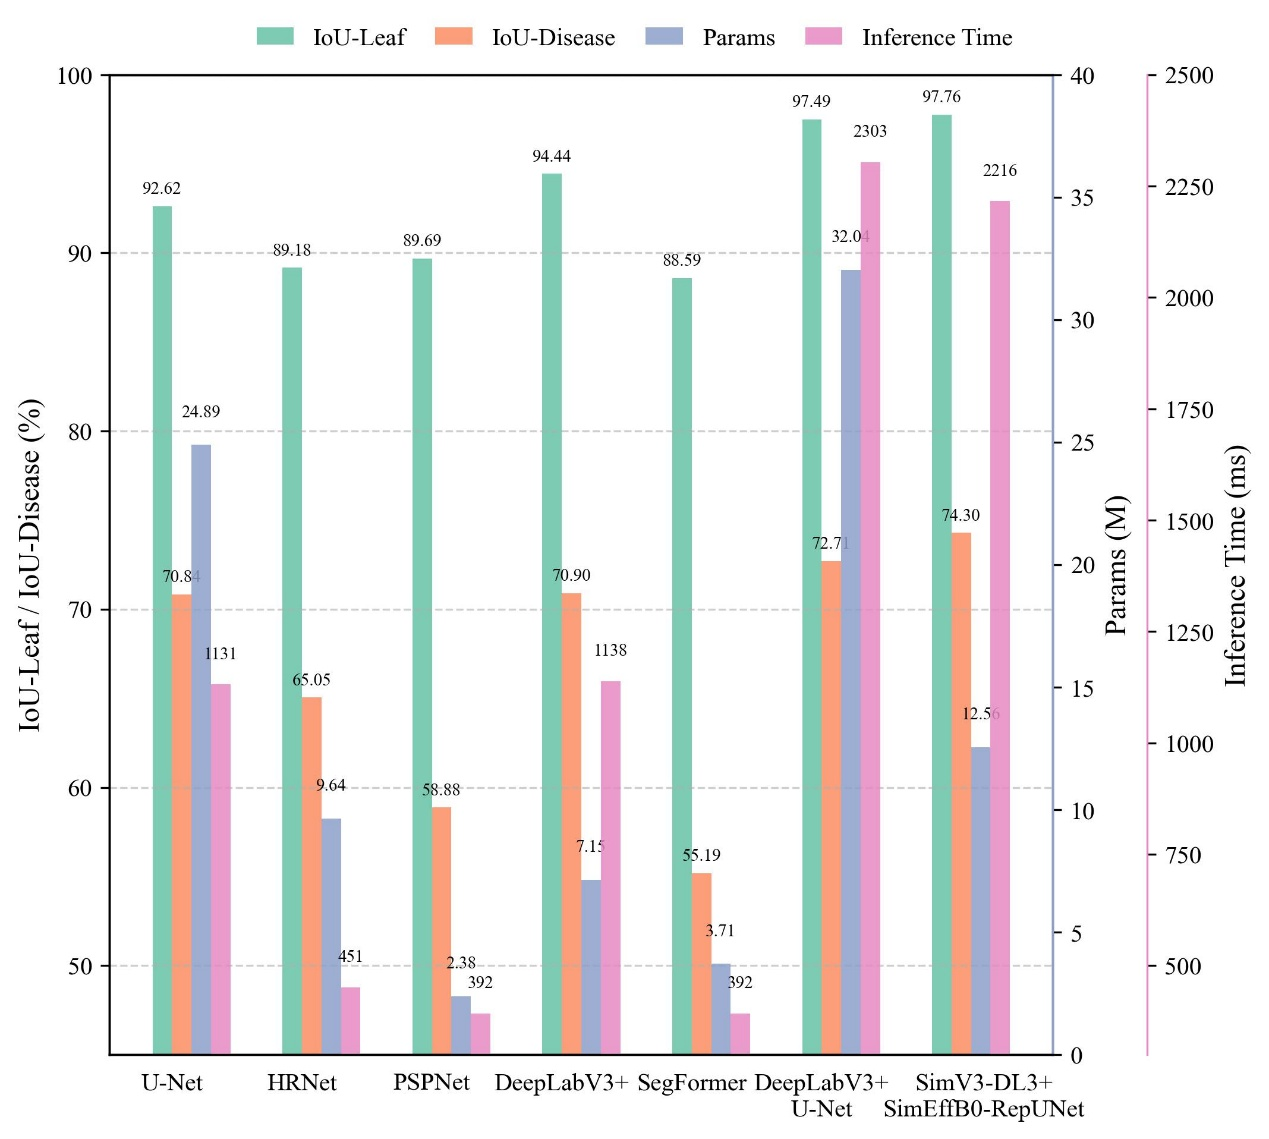
\includegraphics[width=\linewidth]{DSLL-Net-media/media/image10.jpeg}

\hypertarget{fig:10}{}Fig. 10. Performance comparison of single-stage and dual-stage
segmentation models.

\hypertarget{expert-visual-evaluation-and-model-prediction-1}{%
\subsection{Expert Visual Evaluation and Model
Prediction}\label{expert-visual-evaluation-and-model-prediction-1}}

Expert visual estimates showed clear inter-observer variability (Fig.
S3). For a mildly diseased leaf, the mean expert estimate was 4.56\%,
whereas the model predicted 2.32\%. For a more severely diseased leaf,
the mean expert estimate (20.01\%) was close to the model prediction
(19.32\%). These results indicate that automated estimation can reduce
subjectivity, particularly under mild disease conditions.

The difference between expert and model estimates was more pronounced
for mild symptoms, where small lesions are easily overestimated by visual
inspection. Under higher severity, the symptomatic area is more apparent
and expert estimates became more concentrated. This pattern supports the
value of pixel-level quantification for early-stage disease monitoring,
where visual scoring is often less stable.

\hypertarget{discussion}{%
\section{Discussion}\label{discussion}}

The results demonstrate that separating leaf and lesion segmentation is
effective for disease severity quantification under field conditions.
The first stage provides a reliable leaf area for severity calculation,
while the second stage focuses on small and irregular symptomatic
regions. Compared with single-stage models, this task decomposition
reduces feature interference and improves the stability of lesion
delineation and severity estimation.

\hypertarget{attention-guided-lightweight-leaf-segmentation-for-robust-field-conditions}{%
\subsection{Attention-guided lightweight leaf segmentation for robust field
conditions}\label{attention-guided-lightweight-leaf-segmentation-for-robust-field-conditions}}

The leaf segmentation results show that DeepLabV3+ with a
SimAM-enhanced MobileNetV3 backbone improves boundary extraction while
keeping the model compact. Attention-guided segmentation studies
\textcolor{blue}{\hyperlink{ref:39}{[39]}, \hyperlink{ref:40}{[40]}} also
show that spatially focused feature enhancement helps suppress
background interference and reduce over-segmentation. This is important because errors in leaf area
directly propagate to severity estimation.

The high IoU-Leaf obtained by SimV3-DL3+ indicates that the first stage
can provide a stable denominator for severity calculation. In visual
results, inaccurate leaf masks often include background pixels or miss
leaf margins, which changes the estimated total leaf area and biases the
final severity ratio. Therefore, a compact but accurate first-stage model
is not only an auxiliary preprocessing step but a key component of the
severity estimation pipeline. This requirement is consistent with recent
resource-constrained recognition and weakly supervised segmentation
workflows \textcolor{blue}{\hyperlink{ref:41}{[41]}, \hyperlink{ref:42}{[42]}}.

\hypertarget{lesion-segmentation-model-performance-enhancement}{%
\subsection{Lesion segmentation model performance
enhancement}\label{lesion-segmentation-model-performance-enhancement}}

For lesion segmentation, the performance gains arise from the combined
use of EfficientNet-B0 \hyperlink{ref:22}{\textcolor{blue}{[22]}}, SimAM,
and RepConv \hyperlink{ref:23}{\textcolor{blue}{[23]}}. EfficientNet-B0
provides a compact encoder for multi-scale lesion features, SimAM
improves spatial localization of small symptoms, and RepConv strengthens
boundary reconstruction during training while preserving inference
efficiency. Together, these components improve IoU-Disease and mIoU
without the large parameter cost of heavier U-Net variants.

The ablation results also show that the lesion stage cannot be optimized
by simply selecting the most compact model. Disease lesions occupy a
small and irregular portion of the image, so excessive compression can
reduce sensitivity to weak symptoms. The proposed SimEffB0-RepUNet
therefore keeps the U-Net encoder--decoder structure but replaces its
heavier components with more efficient alternatives, preserving lesion
detail while reducing parameter count. This design also aligns with
U-Net-based segmentation work using squeeze-and-excitation enhancement
\hyperlink{ref:43}{\textcolor{blue}{[43]}}, dilated attention modules
\hyperlink{ref:44}{\textcolor{blue}{[44]}}, and multi-scale coordinate
attention \hyperlink{ref:45}{\textcolor{blue}{[45]}} for agricultural target
delineation.

\hypertarget{performance-of-the-dual-stage-model}{%
\subsection{Performance of the dual-stage
model}\label{performance-of-the-dual-stage-model}}

The comparison with single-stage and conventional dual-stage models
confirms that independent optimization of leaf and lesion segmentation is
beneficial. The proposed framework improves both leaf and lesion IoU
while using fewer parameters than the DeepLabV3+ + U-Net baseline. Similar
dual-stage disease severity studies based on leaf--lesion decomposition
\textcolor{blue}{\hyperlink{ref:17}{[17}-\hyperlink{ref:19}{19]}} and
crop disease quantification \textcolor{blue}{\hyperlink{ref:46}{[46]},
\hyperlink{ref:47}{[47]}} also support this design logic. This also
explains the strong agreement between predicted and reference severity
values.

This result highlights the main advantage of DSLL-Net: the two stages
solve different visual problems. Leaf segmentation emphasizes global
shape and background separation, whereas lesion segmentation emphasizes
local texture and boundary refinement. Prior segmentation and dual-stage
severity-estimation studies \textcolor{blue}{\hyperlink{ref:16}{[16}-\hyperlink{ref:19}{19]}}
show similar benefits from separating symptom delineation from whole-leaf
context. By allowing each model to focus on one task, DSLL-Net reduces
conflicting feature requirements and improves the reliability of
downstream severity estimates.

\hypertarget{practical-deployment-and-applications}{%
\subsection{Practical deployment and
applications}\label{practical-deployment-and-applications}}

To support field use, the model was integrated into a Flutter-based
Android application (\url{https://github.com/SmartAG-NWAFU/Grape-Downy}).
This implementation demonstrates the feasibility of deploying the
proposed framework for portable disease monitoring and decision support.
Related mobile disease assessment \hyperlink{ref:19}{\textcolor{blue}{[19]}}
and lightweight field-recognition systems
\textcolor{blue}{\hyperlink{ref:41}{[41]}, \hyperlink{ref:42}{[42]}} indicate
that compact segmentation models can be embedded into practical field
tools.

The application workflow follows the same logic as the experimental
pipeline: users acquire or select a leaf image, the system predicts the
leaf mask and lesion mask, and the severity value is calculated from the
two predicted areas. Although further acceleration is required for
large-scale real-time scouting, this prototype shows that the proposed
model can be embedded into an operational tool rather than remaining
only an offline algorithm.

\hypertarget{limitations}{%
\subsection{Limitations}\label{limitations}}

Several limitations remain. DSLL-Net uses two networks and is therefore
slower than some single-stage alternatives. The current evaluation
focuses on one crop-disease system, so broader validation across crops,
diseases, sensors, and field environments is needed. Pixel-level
annotation is also labor-intensive; semi-supervised or weakly supervised
learning may reduce this cost. Finally, severity is estimated from lesion
area alone, and future work may incorporate temporal or multispectral
information.

Additional implementation details, complete ablation settings, and
qualitative examples can be provided in the Supplementary Materials to
keep the main text concise while preserving reproducibility.

In future work, the framework should be evaluated on images collected
under broader illumination conditions, growth stages, and disease
pressures. Multi-leaf image processing and temporal severity tracking
would also increase its value for field-scale disease monitoring.
Combining RGB imagery with additional sensing modalities may further
improve severity estimation when symptoms are weak or partially
occluded.

\hypertarget{conclusion}{%
\section{Conclusion}\label{conclusion}}

This study proposes DSLL-Net, a lightweight dual-stage framework for
grapevine downy mildew severity assessment. SimV3-DL3+ extracts leaf
regions from field backgrounds, while SimEffB0-RepUNet segments small
and irregular lesions using a SimAM-EfficientNet-B0 encoder and RepConv
decoder. The final model achieved 74.3\% IoU-Disease with 12.56 M
parameters and produced severity estimates highly consistent with
reference values (\(R^{2}=0.976\)). These results indicate that DSLL-Net
provides an efficient and deployable solution for quantitative disease
monitoring. Future work will expand validation across more crops,
diseases, and field conditions and further optimize edge-device
deployment.

\hypertarget{data-and-code-availability}{%
\section*{Data and code availability}\label{data-and-code-availability}}

The data and code used in this study are available on GitHub
(\url{https://github.com/SmartAG-NWAFU/Grape-Downy}).

\hypertarget{author-contribution-statement}{%
\section*{Author contribution
statement}\label{author-contribution-statement}}

Changqing Yan, Gang Zhao: Writing -- review \& editing, Validation,
Supervision, Resources, Project administration, Methodology, Funding
acquisition, Conceptualization. Shuyang Li: Writing -- original draft,
Visualization, Validation, Methodology, Data curation,
Conceptualization. Ling Yin: Supervision, project administration,
funding acquisition. Zhe Liu, Shumei Wei, Xin Lin, Xin Li, Jindong Liu,
Zhenpeng Huang, Danni Zheng, Zeyun Liang, Linjia Yao, Bin Chen, Qi Tian:
Data curation, Investigation, Validation, Writing -- review \& editing.
Chenliang Wang, Junjie Qu: Writing -- review \& editing, Visualization,
Validation, Data curation.

\hypertarget{declaration-of-competing-interest}{%
\section*{Declaration of competing
interest}\label{declaration-of-competing-interest}}

The authors declare that they have no known competing financial
interests or personal relationships that could have appeared to
influence the work reported in this paper.

\hypertarget{acknowledgments}{%
\section*{Acknowledgments}\label{acknowledgments}}

The authors gratefully acknowledge financial support from the Key
Research and Development Program of Shaanxi (Grant No. 2023-ZDLNY-64),
Guangxi Key R\&D Program Project (Grant No. Gui Ke AB24010121).

\hypertarget{supplementary-materials}{%
\section*{Supplementary Materials}\label{supplementary-materials}}

\hypertarget{fig:S1}{}\hypertarget{fig:S2}{}\hypertarget{fig:S3}{}\hypertarget{fig:S4}{}Figs.S1-Figs.S4: Fig.S1 Fig.S2 Fig.S3 Fig.S4.

\hypertarget{references}{%
\section*{References}\label{references}}

\hypertarget{ref:1}{\textcolor{blue}{[1]}} L. Guo \emph{et al.}, ``Super pangenome of Vitis empowers
identification of downy mildew resistance genes for grapevine
improvement,'' \emph{Nature Genetics}, vol. 57, no. 3, pp. 741--753,
Mar. 2025, doi: 10.1038/s41588-025-02111-7.

\hypertarget{ref:2}{\textcolor{blue}{[2]}} L. Bin, Z. Ding, L.
Tian, D. He, S. Li, and H. Wang, ``Grape Leaf Disease Identification
Using Improved Deep Convolutional Neural Networks,'' \emph{Frontiers in
Plant Science}, vol. 11, p. 1082, Jul. 2020, doi:
10.3389/fpls.2020.01082.

\hypertarget{ref:3}{\textcolor{blue}{[3]}} W. Hui \emph{et al.}, ``Adoption of
Sobol's analysis method improved the application of a coupled primary
and secondary infection grape downy mildew model in northern China,''
\emph{Computers and Electronics in Agriculture}, vol. 199, p. 107154,
2022, doi: https://doi.org/10.1016/j.compag.2022.107154.

\hypertarget{ref:4}{\textcolor{blue}{[4]}} S.
Savary, A. Ficke, J.-N. Aubertot, and C. Hollier, ``Crop losses due to
diseases and their implications for global food production losses and
food security,'' \emph{Food security}, vol. 4, no. 4, pp. 519--537,
2012.

\hypertarget{ref:5}{\textcolor{blue}{[5]}} Y. Wang \emph{et al.}, ``High-efficiency fungicide
screening and field control efficacy of maize southern corn rust,''
\emph{Crop Protection}, vol. 187, p. 106997, 2025.

\hypertarget{ref:6}{\textcolor{blue}{[6]}} M. Ji, L.
Zhang, and Q. Wu, ``Automatic grape leaf diseases identification via
UnitedModel based on multiple convolutional neural networks,''
\emph{Information Processing in Agriculture}, vol. 7, no. 3, pp.
418--426, 2020, doi: https://doi.org/10.1016/j.inpa.2019.10.003.

\hypertarget{ref:7}{\textcolor{blue}{[7]}}N. R. Kolhalkar and V. L. Krishnan, ``Mechatronics system for diagnosis
and treatment of major diseases in grape vineyards based on image
processing,'' \emph{Materials Today: Proceedings}, vol. 23, pp.
549--556, 2020, doi: https://doi.org/10.1016/j.matpr.2019.05.407.

\hypertarget{ref:8}{\textcolor{blue}{[8]}}L. I. Cazón, J. A. Paredes, N. R. González, E. C. Conforto, L. Suarez,
and E. M. Del Ponte, ``Optimizing visual estimation of peanut late leaf
spot severity with online training sessions and standard area
diagrams,'' \emph{European Journal of Plant Pathology}, pp. 1--15,
2025.

\hypertarget{ref:9}{\textcolor{blue}{[9]}} T. Shi \emph{et al.}, ``Recent advances in plant disease
severity assessment using convolutional neural networks,''
\emph{Scientific Reports}, vol. 13, no. 1, p. 2336, Feb. 2023, doi:
10.1038/s41598-023-29230-7.

\hypertarget{ref:10}{\textcolor{blue}{[10]}} K. Li, L. Zhang, B. Li, S. Li, and
J. Ma, ``Attention-optimized DeepLab V3\,+\,for automatic estimation of
cucumber disease severity,'' \emph{Plant Methods}, vol. 18, no. 1, p.
109, Sep. 2022, doi: 10.1186/s13007-022-00941-8.

\hypertarget{ref:11}{\textcolor{blue}{[11]}} J. G. M.
Esgario, R. A. Krohling, and J. A. Ventura, ``Deep learning for
classification and severity estimation of coffee leaf biotic stress,''
\emph{Computers and Electronics in Agriculture}, vol. 169, p. 105162,
2020, doi: https://doi.org/10.1016/j.compag.2019.105162.

\hypertarget{ref:12}{\textcolor{blue}{[12]}} I.
Hernández \emph{et al.}, ``Assessment of downy mildew in grapevine using
computer vision and fuzzy logic. Development and validation of a new
method,'' \emph{OENO One}, vol. 56, no. 3, pp. 41--53, Jul. 2022, doi:
10.20870/oeno-one.2022.56.3.5359.

\hypertarget{ref:13}{\textcolor{blue}{[13]}} Q. Liang, S. Xiang, Y. Hu, G.
Coppola, D. Zhang, and W. Sun, ``PD2SE-Net: Computer-assisted plant
disease diagnosis and severity estimation network,'' \emph{Computers and
Electronics in Agriculture}, vol. 157, pp. 518--529, 2019, doi:
https://doi.org/10.1016/j.compag.2019.01.034.

\hypertarget{ref:14}{\textcolor{blue}{[14]}} Z. Wang, L. Yang,
R. Wang, L. Lei, H. Ding, and Q. Yang, ``WE-DeepLabV3+: A lightweight
segmentation model for Panax notoginseng leaf diseases,''
\emph{Computers and Electronics in Agriculture}, vol. 227, p. 109612,
2024, doi: https://doi.org/10.1016/j.compag.2024.109612.

\hypertarget{ref:15}{\textcolor{blue}{[15]}} C. Zhao
\emph{et al.}, ``Plant Disease Segmentation Networks for Fast Automatic
Severity Estimation Under Natural Field Scenarios,'' \emph{Agriculture},
vol. 15, no. 6, 2025, doi: 10.3390/agriculture15060583.

\hypertarget{ref:16}{\textcolor{blue}{[16]}} I.
Hernández, R. Silva, P. Melo-Pinto, S. Gutiérrez, and J. Tardaguila,
``Early detection of downy mildew in vineyards using deep neural
networks for semantic segmentation,'' \emph{Biosystems Engineering},
vol. 252, pp. 15--31, 2025, doi:
https://doi.org/10.1016/j.biosystemseng.2025.02.007.

\hypertarget{ref:17}{\textcolor{blue}{[17]}} C. Wang, P.
Du, H. Wu, J. Li, C. Zhao, and H. Zhu, ``A cucumber leaf disease
severity classification method based on the fusion of DeepLabV3+ and
U-Net,'' \emph{Computers and Electronics in Agriculture}, vol. 189, p.
106373, 2021, doi: https://doi.org/10.1016/j.compag.2021.106373.

\hypertarget{ref:18}{\textcolor{blue}{[18]}}Y. Xu \emph{et al.}, ``Accurate cotton verticillium wilt segmentation in
field background based on the two-stage lightweight DeepLabV3+ model,''
\emph{Computers and Electronics in Agriculture}, vol. 229, p. 109814,
2025, doi: https://doi.org/10.1016/j.compag.2024.109814.

\hypertarget{ref:19}{\textcolor{blue}{[19]}} W. Liu \emph{et al.}, ``StripeRust-Pocket: A
Mobile-Based Deep Learning Application for Efficient Disease Severity
Assessment of Wheat Stripe Rust,'' \emph{Plant Phenomics}, vol. 6, p.
0201, 2024, doi: 10.34133/plantphenomics.0201.

\hypertarget{ref:20}{\textcolor{blue}{[20]}} L.-C. Chen,
Y. Zhu, G. Papandreou, F. Schroff, and H. Adam, ``Encoder-Decoder with
Atrous Separable Convolution for Semantic Image Segmentation,'' Aug. 22,
2018, \emph{arXiv}: arXiv:1802.02611. doi:
10.48550/arXiv.1802.02611.

\hypertarget{ref:21}{\textcolor{blue}{[21]}} A. Howard \emph{et al.}, ``Searching
for MobileNetV3,'' in \emph{2019 IEEE/CVF International Conference on
Computer Vision (ICCV)}, 2019, pp. 1314--1324. doi:
10.1109/ICCV.2019.00140.

\hypertarget{ref:22}{\textcolor{blue}{[22]}} C. Lin, P. Yang, Q. Wang, Z. Qiu, W. Lv, and
Z. Wang, ``Efficient and accurate compound scaling for convolutional
neural networks,'' \emph{Neural Networks}, vol. 167, pp. 787--797,
2023.

\hypertarget{ref:23}{\textcolor{blue}{[23]}} X. Ding, X.
Zhang, N. Ma, J. Han, G. Ding, and J. Sun, ``RepVGG: Making VGG-style
ConvNets Great Again,'' in \emph{2021 IEEE/CVF Conference on Computer
Vision and Pattern Recognition (CVPR)}, 2021, pp. 13728--13737. doi:
10.1109/CVPR46437.2021.01352.

\hypertarget{ref:24}{\textcolor{blue}{[24]}} V. Iglovikov and A. Shvets,
``TernausNet: U-Net with VGG11 Encoder Pre-Trained on ImageNet for Image
Segmentation,'' 2018, \emph{arXiv}: arXiv:1801.05746. doi:
10.48550/arXiv.1801.05746.

\hypertarget{ref:25}{\textcolor{blue}{[25]}} H. Zhao, J. Shi, X. Qi, X. Wang, and
J. Jia, ``Pyramid Scene Parsing Network,'' in \emph{2017 IEEE Conference
on Computer Vision and Pattern Recognition (CVPR)}, 2017, pp.
6230--6239. doi: 10.1109/CVPR.2017.660.

\hypertarget{ref:26}{\textcolor{blue}{[26]}} E. Xie, W. Wang, Z. Yu,
A. Anandkumar, J. M. Alvarez, and P. Luo, ``SegFormer: simple and
efficient design for semantic segmentation with transformers,'' in
\emph{Proceedings of the 35th International Conference on Neural
Information Processing Systems}, in NIPS '21. Red Hook, NY, USA: Curran
Associates Inc., 2021.

\hypertarget{ref:27}{\textcolor{blue}{[27]}} J. Wang \emph{et al.}, ``Deep
High-Resolution Representation Learning for Visual Recognition,''
\emph{IEEE Transactions on Pattern Analysis and Machine Intelligence},
vol. 43, no. 10, pp. 3349--3364, 2021, doi:
10.1109/TPAMI.2020.2983686.

\hypertarget{ref:28}{\textcolor{blue}{[28]}} M. Sandler, A. Howard, M. Zhu, A.
Zhmoginov, and L.-C. Chen, ``MobileNetV2: Inverted Residuals and Linear
Bottlenecks,'' in \emph{2018 IEEE/CVF Conference on Computer Vision and
Pattern Recognition}, 2018, pp. 4510--4520. doi:
10.1109/CVPR.2018.00474.

\hypertarget{ref:29}{\textcolor{blue}{[29]}} D. Qin \emph{et al.}, ``MobileNetV4:
Universal Models for Mobile Ecosystem,'' in \emph{Computer Vision --
ECCV 2024: 18th European Conference, Milan, Italy, September 29--October
4, 2024, Proceedings, Part XL}, Berlin, Heidelberg: Springer-Verlag,
2024, pp. 78--96. doi: 10.1007/978-3-031-73661-2\_5.

\hypertarget{ref:30}{\textcolor{blue}{[30]}} J. Hu, L.
Shen, and G. Sun, ``Squeeze-and-Excitation Networks,'' in \emph{2018
IEEE/CVF Conference on Computer Vision and Pattern Recognition}, 2018,
pp. 7132--7141. doi: 10.1109/CVPR.2018.00745.

\hypertarget{ref:31}{\textcolor{blue}{[31]}} L. Yang, R.-Y.
Zhang, L. Li, and X. Xie, ``SimAM: A Simple, Parameter-Free Attention
Module for Convolutional Neural Networks,'' in \emph{International
Conference on Machine Learning}, 2021. {[}Online{]}. Available:
https://api.semanticscholar.org/CorpusID:235825945

\hypertarget{ref:32}{\textcolor{blue}{[32]}} X. Ma, X. Dai, Y. Bai, Y. Wang,
and Y. Fu, ``Rewrite the Stars,'' in \emph{2024 IEEE/CVF Conference on
Computer Vision and Pattern Recognition (CVPR)}, 2024, pp. 5694--5703.
doi: 10.1109/CVPR52733.2024.00544.

\hypertarget{ref:33}{\textcolor{blue}{[33]}} K. He, X. Zhang, S. Ren, and
J. Sun, ``Deep Residual Learning for Image Recognition,'' in \emph{2016
IEEE Conference on Computer Vision and Pattern Recognition (CVPR)},
2016, pp. 770--778. doi: 10.1109/CVPR.2016.90.

\hypertarget{ref:34}{\textcolor{blue}{[34]}} Q. Wang, B. Wu,
P. Zhu, P. Li, W. Zuo, and Q. Hu, ``ECA-Net: Efficient Channel Attention
for Deep Convolutional Neural Networks,'' in \emph{2020 IEEE/CVF
Conference on Computer Vision and Pattern Recognition (CVPR)}, 2020, pp.
11531--11539. doi: 10.1109/CVPR42600.2020.01155.

\hypertarget{ref:35}{\textcolor{blue}{[35]}} S. Woo, J.
Park, J.-Y. Lee, and I. S. Kweon, ``CBAM: Convolutional Block Attention
Module,'' in \emph{Computer Vision -- ECCV 2018: 15th European
Conference, Munich, Germany, September 8--14, 2018, Proceedings, Part
VII}, Berlin, Heidelberg: Springer-Verlag, 2018, pp. 3--19. doi:
10.1007/978-3-030-01234-2\_1.

\hypertarget{ref:36}{\textcolor{blue}{[36]}} L. Bai and Z. J. Song,
``Omni-dimensional dynamic convolution with coordinate attention
detection scheme,'' \emph{Science Progress}, vol. 108, no. 2, p.
00368504251336695, 2025, doi: 10.1177/00368504251336695.

\hypertarget{ref:37}{\textcolor{blue}{[37]}} J. Chen
\emph{et al.}, ``Run, Don't Walk: Chasing Higher FLOPS for Faster Neural
Networks,'' in \emph{2023 IEEE/CVF Conference on Computer Vision and
Pattern Recognition (CVPR)}, 2023, pp. 12021--12031. doi:
10.1109/CVPR52729.2023.01157.

\hypertarget{ref:38}{\textcolor{blue}{[38]}} B. Yang, G. Bender, Q. V. Le, and
J. Ngiam, ``CondConv: conditionally parameterized convolutions for
efficient inference,'' in \emph{Proceedings of the 33rd International
Conference on Neural Information Processing Systems}, Red Hook, NY, USA:
Curran Associates Inc., 2019.

\hypertarget{ref:39}{\textcolor{blue}{[39]}} X. Dong \emph{et al.}, ``Detection
of pine wilt disease infected pine trees using YOLOv5 optimized by
attention mechanisms and loss functions,'' \emph{Ecological Indicators},
vol. 168, p. 112764, Nov. 2024, doi:
10.1016/j.ecolind.2024.112764.

\hypertarget{ref:40}{\textcolor{blue}{[40]}} F. Wen \emph{et al.}, ``Accurate
recognition and segmentation of northern corn leaf blight in drone RGB
Images: A CycleGAN-augmented YOLOv5-Mobile-Seg lightweight network
approach,'' \emph{Computers and Electronics in Agriculture}, vol. 236,
p. 110433, Sep. 2025, doi: 10.1016/j.compag.2025.110433.

\hypertarget{ref:41}{\textcolor{blue}{[41]}} J. Zi,
W. Hu, G. Fan, F. Chen, and Y. Chen, ``SFL-MobileNetV3: A lightweight
network for weed recognition in tropical cassava fields in China,''
\emph{Expert Systems with Applications}, vol. 277, p. 127196, 2025, doi:
https://doi.org/10.1016/j.eswa.2025.127196.

\hypertarget{ref:42}{\textcolor{blue}{[42]}} M. Parajuli, M.
Shaban, and T. L. Phung, ``Automated differentiation of skin melanocytes
from keratinocytes in high-resolution histopathology images using a
weakly-supervised deep-learning framework,'' \emph{Int. J. Imaging Syst.
Technol.}, vol. 33, pp. 262-\/-275, 2023, doi:
10.1002/IMA.22810.

\hypertarget{ref:43}{\textcolor{blue}{[43]}} B. Zhang \emph{et al.}, ``Multi-scale segmentation
squeeze-and-excitation UNet with conditional random field for segmenting
lung tumor from CT images,'' \emph{Computer Methods and Programs in
Biomedicine}, vol. 222, p. 106946, 2022.

\hypertarget{ref:44}{\textcolor{blue}{[44]}} C. Zhang, Y. Zhang, and
X. Xu, ``Dilated inception U-Net with attention for crop pest image
segmentation in real-field environment,'' \emph{Smart Agricultural
Technology}, vol. 11, p. 100917, Aug. 2025, doi:
10.1016/j.atech.2025.100917.

\hypertarget{ref:45}{\textcolor{blue}{[45]}} R. Gu and L. Liu, ``An agricultural
leaf disease segmentation model applying multi-scale coordinate
attention mechanism,'' \emph{Applied Soft Computing}, vol. 172, p.
112904, Mar. 2025, doi: 10.1016/j.asoc.2025.112904.

\hypertarget{ref:46}{\textcolor{blue}{[46]}} L. G.
Divyanth, A. Ahmad, and D. Saraswat, ``A two-stage deep-learning based
segmentation model for crop disease quantification based on corn field
imagery,'' \emph{Smart Agricultural Technology}, vol. 3, p. 100108,
2023, doi: https://doi.org/10.1016/j.atech.2022.100108.

\hypertarget{ref:47}{\textcolor{blue}{[47]}} B.-Y.
Liu, K.-J. Fan, W.-H. Su, and Y. Peng, ``Two-Stage Convolutional Neural
Networks for Diagnosing the Severity of Alternaria Leaf Blotch Disease
of the Apple Tree,'' \emph{Remote Sensing}, vol. 14, no. 11, 2022, doi:
10.3390/rs14112519.

\end{document}
